\documentclass{article}

\usepackage{frongillo}

\title{\textbf{Orale di italiano\\Corso Passerella}}
\author{Matteo Frongillo, Paolo Bettelini}

\begin{document}

\maketitle
\tableofcontents
\phantom{}
\pagebreak


%%%%%%%%%%%%%%%
\paragraph*{Suddivisione testi}

\textbf{Paolo}
\begin{itemize}
    \item Dante Alighieri (Oltre la spera, Inferno I, Inferno III);
    \item Machiavelli (Sintesi della vita di Machiavelli, Lettera al Vettori, Dedica, Capitoli I, VI, XV, XVIII, XXV);
    \item Ariosto (Vita di Ariosto con personaggi esterni [Ippolito, Alessandra, Boiardo] , Canti I, XIX, XXIII)
    \item Pietro Verri (Spiegare l'illuminismo e il Caffé, Lettera agli amici milanesi);
    \item Beccaria (Capitoli I, VI, XII).
\end{itemize}

\textbf{Matteo}
\begin{itemize}
    \item Petrarca (Struttura di Rvf, vita di Petrarca, Capitoli I, III, XVI, XXII, XC, CCCX);
    \item Boccaccio (Struttura del Decameron, Peste, Novelle II.5, III.2, IV.5, V.8, VI.10, VII.1);
    \item Leopardi (Spiego l'illuminismo e il pessimismo, Islandese, Venditore d'almanacchi, L'Infinito, La quiete dopo la tempesta, Sabato del villaggio).
\end{itemize}

%%%%%%%%%%%%

\newpage
\part{Esami scritti}

\section{Come analizzare in base all'autore}
\textbf{Dante}
\begin{itemize}
    \item Passo di un canto della \textit{Commedia} o prosimetro della \textit{Vita nova};
    \item Seguire il testo dalla lettera al concetto;
    \item Fare analogie con gli altri canti.
\end{itemize}

\textbf{Boccaccio}
\begin{itemize}
    \item Novella del \textit{Decameron};
    \item Seguire tutto il testo passo passo;
    \item Analisi a livelli:
        \begin{itemize}
            \item Analisi dei personaggi;
            \item Analisi degli spazi e dei tempi se necessario;
        \end{itemize}
    \item Arrivare al sistema di valori che sta dietro alla novella;
    \item Fare attenzione alla struttura del testo:
        \begin{itemize}
            \item Rubrica;
            \item Cornice;
            \item Coordinata ideologica spesso relativa ad altre novelle;
        \end{itemize}
    \item Fare analogie con le altre novelle.
\end{itemize}

\textbf{Petrarca}
\begin{itemize}
    \item Canto del \textit{Rerum vulgarium fragmenta};
    \item Spiegare di cosa parla il testo;
    \item Analisi:
        \begin{itemize}
            \item Analizzare strofa per strofa;
            \item Analizzare il testo dal generale allo specifico;
            \item ``Essere / dover essere'' 
        \end{itemize}
    \item Ritornare dall'analisi di ogni strofa al generale di tutto il testo:
        \begin{itemize}
            \item Capire come è strutturato il testo;
            \item Cercare figure retoriche nella struttura:
                \begin{itemize}
                    \item Struttura fatta a climax;
                    \item Struttura fatta a similitudine (``ma'' avversativo);
                \end{itemize}
        \end{itemize}
    \item Dare importanza alle analogie tra i verbi;
    \item Dare importanza all'utilizzo dei diversi tempi verbali.
\end{itemize}

\textbf{Machiavelli}
\begin{itemize}
    \item Capitolo de \textit{Il Principe};
    \item Seguire il testo durante l'analisi;
    \item Ripetere sostanzialmente ciò che dice l'autore, concentrandosi sugli snodi cruciali;
    \item Tenere in considerazione la vita politica di Machiavelli e il suo ruolo importante
        come consigliere;
    \item Riallacciare i discorsi alla sua vita e agli altri testi leggi;
    \item Citare il testo (per gli scritti).
\end{itemize}

\textbf{Beccaria e Verri}
\begin{itemize}
    \item Capitolo di \textit{Dei delitti e delle pene};
    \item Seguire il testo durante l'analisi;
    \item Ripetere sostanzialmente ciò che dice l'autore, concentrandosi sugli snodi cruciali;
    \item Tenere in considerazione la vita di Beccaria e il ruolo de \textit{Il Caffé};
    \item Riallacciare i discorsi alla sua vita e agli altri testi leggi;
    \item Citare il testo (per gli scritti).

\end{itemize}

\textbf{Ariosto}
\begin{itemize}
    \item Passo di un canto dell'\textit{Orlando furioso};
    \item Parlare in generale di cosa tratta il passo;
    \item Analizzare ogni ottava dal generale allo specifico;
    \item Correlare il passo agli altri canti letti.
\end{itemize}

\textbf{Leopardi}
\begin{itemize}
    \item Canto di \textit{Canti} oppure opera delle \textit{Operette morali};
    \item Trattare i temi legati alla ragione della vita, pessimismo e Natura impersonificata;
    \item Riflessioni sulla vita;
    \item Analisi accompagnata da passi dello \textit{Zibaldone};
    \item Correlare il canto o l'opera alle altre viste e ai passi dello \textit{Zibaldone}.
\end{itemize}

%%%%%%%%%%%%

\newpage

\part{Esame Orale}

\section{Dante Alighieri}

\subsection{Vita nova}

\begin{enumerate}
    \item Vita nova è il primo prosimetro di Dante
    \item Racconta la storia d'amore di Dante per Beatrice;
    \item Questa vicenda diventa un modello per questa tipologia di narrativa
    \item Il titolo indica come Dante consideri l’inizio della sua vita (nuova vita, rinnovata) quando
    vide Beatrice per la prima volta.
    \item Il primo contatto amoroso nella poesie è spesso caratterizzato da un
    innamoramento a prima vista.
    \item Quando la voce dell’interesse di Dante nei confronti di Beatrice le giunge, lei gli nega il saluto.
    \item Il saluto nel medioevo ha un significato molto più profondo di quello odierno.
    \item Nonostante il rifiuto, Dante continua ad esprimere il suo amore verso Beatrice semplicemente lodandola
    (scrivendo di lei), completamente senza ricambio di interesse
    \item Questa loda rappresenta la forma più pura di amore.
    \item Questo libro introduce la simbologia del numero 9 associato a Beatrice. Ciò è dato dal fatto che Dante
    l’abbia vista per la prima volta a 9 anni, rivista 9 anni dopo, e altri motivi che vengono descritti. Il numero
    9 è anche un simbolo biblico (3 volte la trinità).
\end{enumerate}

\subsubsection{Oltre la spera che più larga gira}

\begin{enumerate}
    \item È l'ultimo sonetto di Vita nova, il libro che racconta la storia d'amore di Dante
    per Beatrice.
    \item È importante considerare il significato del titolo di Vita nova (vedi prima).
    \item Questo sonetto descrive il concetto di intelligenza nova indotta nello spirito di Dante.
    \item Il primo verso è una perifrasi che indica “oltre il corpo celeste più lontano” (chiamato Il Primo Mobile), ossia il
    paradiso siccome la visione dell’universo era quella tolemaica e creazionista.
    \item Per contestualizzare è necessario parlare del sistema tolemaico (di Claudio Tolomeo), ossia il sistema geocentrico.
    \item Secondo questo sistema, la terra è fissa al centro degli universo (elemento antropocentrista)
    \item Attorno, I vari pianeti ruotano attorno alla terra in delle orbite circolari sempre più distanti
    \item Questi corpi celesti sono trascinati da delle sfere di cristallo (ossia un manteriale perfetto, indistruttibile).
    \item Queste credenze derivano dalla Genesi, il primo libro della Bibbia, che descrive la creazione del mondo da parte di Dio in sei giorni.
    \item Dalla descrizione del firmamento della bibbia, ossia quello di essere come una cupola, nasce l'idea di sfere di cristallo che sostengono i corpi celesti.
    \item Il Primo Mobile rappresenta quindi la sfera più esterna dell'universo, che contiene tutte le stelle fisse.
    \item oltre il Primo Mobile, vi è il paradiso con Dio. Ed è proprio questo al quale Dante sta facendo riferimento (oltre l'ultima sfera)
    \item Il secondo verso ci indica che il sospiro del poeta esce dal suo cuore, mentre è vivo, dalla sua intimità più
    profonda, e attraverso i cieli fino al paradiso.
    \item Ai versi 3-4 viene descritto ciò che permette questo percorso, ossia ciò che lo tira verso l’alto.
    \item Questa forza è un’intelligenza nova, ossia una nuova sensibilità nel vedere le cose.
    \item Questa nuova intelligenza deriva dall’amore, che permette all’autore di avere una nuova consapevolezza.
    \item L'sperienza amorosa è dolorosama porta ad una nuova capacità di intendimento. 
    \item Amore personificato con la A maiuscola, classico elemento del dolce Stilnovo.
    \item La seconda quartina descrive il punto di arrivo.
    \item Quando lo spirito arriva, vede una donna, la quale viene
    onorata dagli altri beati, Dio e la Madonna.
    \item Viene anche detto che questa donna brilla (luce è un verbo).
    \item causa di questo grande splendore, lo spirito giunto in paradiso (pellegrino, in pellegrinaggio) la ammira.
    \item Dalla terza quartina Lo spirito ripercorre il medesimo tragitto verticale, ma al contrario, tornando da Dante.
    \item Questo spirito cerca di spiegargli che cosa ha visto. “La vede tale che quando me lo ridice, io non capisco”
    \item Dante non comprende
    quindi ciò che lo spirito gli riferisce, perché “parla sottile”, ossia parla in maniera troppo difficile.
    \item Il cuore dolente del poeta è ciò che fa sì che lo spirito venga interrogato.
    \item Infatti, lo spirito parla proprio al cuore \underline{e} a
    Dante (questo amplifica l’incomprensione della spiegazione)
    \item Lo spirito parla in maniera troppo complessa
    perché il linguaggio non riesce ad esprimere quello che si è provato (topos dell’ineffabilità, è ineffabile) siccome
    l’esperienza lo trascende.
    \item Alla quarta terzina Dante capisce che la donna in questione è Beatrice nonostante l'incomprensione con il suo spirito.
    \item Nella poesia antica, la parola gentile è molto più profonda di quella odierna e possiede un significato diverso, ossia un significato nobile di purezza (nobiltà d'animo).
    \item La parola ``però'' vuol dire ``per ciò''. 
    \item Beatrice viene nominata, una occasione molto rara.
    \item Infinite, l'ultimo verso è dato dal fatto che Dante si stesse riferendo a delle Donne nel testo, quindi non è rilevante.
    \item Nel complesso, il sonetto è diviso in due. Vengono distinte le due verticalità del viaggio, avanti e indietro.
    \item Molte parole della prima parte appartengono alla sfera visiva, poiché il paradiso è fatto di luci
    \item Molte parole della seconda parte riguardando dal sfera del parlare.
    \item Per cui lo spirito può vedere ma ha l'impossibilità di esprimersi.
    \item Questa separazione è collegata dall'uso di due parole quasi uguali, \textbf{mira} e \textbf{Vedela} (detto per anadiplosi).
\end{enumerate}

\newpage
\subsection{La Commedia}
\subsubsection{Inferno I}

--

\newpage
\subsection{La Commedia}
\subsubsection{Inferno III}

--

\newpage
\section{Francesco Petrarca}
\subsection{Canzoniere - Rerum vulgarium fragmenta}
La raccolta è composta da 366 liriche e parla dell'amore tormentato di Petrarca nei confronti
di Laura. Il protagonista dei poemi non sarà però Laura, bensì Petrarca stesso che parla di lei.

La raccolta di liriche è separata in due parti, separate con un foglio bianco tra
l'\underline{Rvf 263} e \underline{Rvf 264}:
\begin{enumerate}[label=Parte \arabic*.]
    \item ``In vita di Madonna Laura'', \underline{Rvf 1-263}:\\
        questa sezione comprende le poesie scritte durante la vita di Laura. Petrarca in questi
        esprime la sua passione, il tormento e l'adorazione nei suoi confronti, riflettendo i
        temi di amore cortese, bellezza ideale e struggimento amoroso. Le poesie variano tra
        sonetti, canzoni, sestine, ballate e madrigali, con una forte enfasi sulla bellezza di
        Laura e il desiderio inappagato del poeta;
    \item ``In morte di Madonna Laura'', \underline{Rvf 264-366}:\\
        dopo la morte di Laura, la seconda parte raccoglie le poesie che Petrarca scrive in
        memoria della sua amata. Questi componimenti sono caratterizzati da un tono più
        malinconico e riflessivo, esplorando temi di perdita, dolore e rimpianto. Il poeta
        riflette sulla caducità della vita, la mortalità e il desidero di redenzione spirituale,
        spostando l'attenzione dalla bellezza terrena di Laura alla sua elevazione celeste.

        Di fatto, Laura muore dall'\underline{Rvf 267}, ma Petrarca lascia un cuscinetto di
        tre liriche \underline{Rvf 264-267} che funge da transizione, il quale prepara il
        lettore al cambiamento di tono e di tema, infatti piano piano inizia a distaccarsi da
        tutto ciò che è terreno. Le tre liriche introducono la malinconia e la riflessione che
        enfatizza il processo di accettazione di Petrarca ed il suo cambiamento interiore.
\end{enumerate}

\newpage
\subsubsection{\textit{Voi ch'ascoltate in rime sparse il suono} (Rvf, I)}
\poetry{
    & \textit{Voi ch’ascoltate in rime sparse il suono}\\
    & \textit{di quei sospiri ond’io nudriva ’l core}\\
    & \textit{in sul mio primo giovenile errore}\\
    \text{4.} & \textit{quand’era in parte altr’uom da quel ch’i’ sono,}\\\\
    & \textit{del vario stile in ch’io piango et ragiono}\\
    & \textit{fra le vane speranze e ’l van dolore,}\\
    & \textit{ove sia chi per prova intenda amore,}\\
    \text{8.} & \textit{spero trovar pietà, nonché perdono.}\\\\
    & \textit{Ma ben veggio or sì come al popol tutto}\\
    & \textit{favola fui gran tempo, onde sovente}\\
    \text{11.} & \textit{di me medesmo meco mi vergogno;}\\\\
    & \textit{et del mio vaneggiar vergogna è ’l frutto,}\\
    & \textit{e ’l pentersi, e ’l conoscer chiaramente}\\
    \text{14.} & \textit{che quanto piace al mondo è breve sogno.}
}

\begin{enumerate}
    \item Questo sonetto fa sia da prologo (introduce il libro) sia da epilogo
        (contiene degli elementi che sono già un bilancio di tutta la raccolta).
    \item Metrica: sonetto (2 quartine 2 terzine di endecasillabi);
    \item Schema rime: ABBA, ABBA, CDE, CDE;
    \item Analisi letterale:
    \begin{itemize}[label=]
        \item \textbf{Prima quartina}
        \begin{enumerate}[label=]
            \citem[v.1]{Voi ch'ascoltate} il sonetto si apre con un'invocazione verso il
            lettore (apostrofe);
        \citem[v.1]{in rime sparse} indica la forma della raccolta, ossia frammenti di
            poesie sparse autonome;
        \citem[vv.1-2]{il suono / di quei sospiri ond'io nudriva 'l core} indica il
            contenuto del canzoniere, infatti questo enjambement indica l'amore;
        \citem[vv.2-3]{in sul mio primo giovenile errore / quand'era in parte altr'uomo da
            quel ch'i' sono,} è l'elemento che fa capire al lettore che questo sonetto non è
            stato scritto prima della raccolta di poesie, infatti esso funge anche da
            \underline{epilogo}, poiché dice che il suo amore che canterà è stato un errore;
        \citem[v.4]{in parte} sta ad indicare che Petrarca non ha ancora superato 
            completamente il suo amore sbagliato;
        \item Le rime \textit{``core / errore''} [vv.2-3] e \textit{``dolore / amore''}
            [vv.6-7], fanno capire che lui considera l'amore provato come un errore e come
            amore non degno, poiché l'unico vero amore terreno dovrebbe essere solo quello nei
            confronti di Dio.

            Dunque, l'amore per una persona terrena è uno sviamento e una distrazione da un
            amore giusto ed eterno.\\
            \phantom{}

            \item \textbf{La conflittualità:}

            Già dalla prima quartina, si nota il conflitto tra l'\textbf{Amore sacro} e
            l'\textbf{Amore profano}, tra il \textbf{Dover essere} e tra l'\textbf{Essere},
            tra il \textbf{Dovere} e il \textbf{Piacere}.

            \emph{Questo conflitto tra cos'è giusto e cos'è meno giusto è il tema principale
            del Canzoniere}.\\
            \phantom{}
        \end{enumerate}

        \newpage
        \item \textbf{Seconda quartina}
            \begin{enumerate}[label=]
                \citem[vv.5-6]{vario stile} si intende la penna che oscilla tra
                    \textit{``piango et ragiono / ...speranze...dolore''}. Queste quattro
                    parole formano un chiasmo:
                        \begin{itemize}
                            \item Le parole esterne ``piango, dolore'' sono quelle che
                                enfatizzano il dolore dell'autore;
                            \item Le parole interne ``ragiono, speranze'' indicano la
                                razionalità e la lucidità della situazione.
                        \end{itemize}
                    \begin{itemize}
                        \item Il dolore e le speranze sono ``vane'', ossia sono qualcosa
                            di effimero,che è destinato a finire;
                        \item È per questo che Petrarca punta sullamore verso l'eterno e non
                            sull'amore terreno, poiché ogni cosa terrena è finita e non fale la
                            pena spenderci emozioni appresso.
                    \end{itemize}

                \citem[vv7-8]{ove sia chi per prova intenda amore, / spero di trovar pietà,
                    nonché perdono.};
                    \begin{itemize}
                        \item Petrarca chiede di ritrovare pietà e perdono da chi conosce il
                            vero significato dell'amore;
                        \item Il gruppo di riferimento si restringe alle persone che hanno
                            amato, ma solo chi ha amato tanto quanto lui;
                    \end{itemize}
                \citem[v.8]{spero} è il verbo principale del primo periodo, il quale si
                    riferisce al ``Voi'' iniziale a verso 1.
            \end{enumerate}

        \textbf{Prima terzina}
            \begin{enumerate}[label=]
                \citem[v.9]{Ma} avversativo. Indica un'opposizione alle due quartine;
                \citem[v.10]{favola} intende i pettegolezzi e gli scandali;
                \citem[vv.9-10]{Ma ben veggio or sì come al popol tutto / favola fui gran
                    tempo, onde sovente}:
                        \begin{itemize}
                            \item Petrarca si rende conto di come il suo amore ossessivo e
                                la sua persona fossero diventati oggetto di pettegolezzi tra
                                le persone nella città;
                            \item Il gruppo di riferimento si allarga con ``popol tutto''.
                        \end{itemize}
                \citem[v11]{di me medesmo meco mi vergogno}:
                    \begin{itemize}
                        \item L'autore si vergogna di sé stesso con sé stesso;
                        \item È presente un'allitterazione: ``di Me MedesMo Meco Mi vergogno'',
                            che sta ad sottolineare quanto lui si vergognasse di questo;
                        \item Questa frase crea un vortice di vergogna che Petrarca ora guarda
                            con distacco.
                    \end{itemize}
            \end{enumerate}
        
        \textbf{Seconda terzina}
            \begin{enumerate}[label=]
                \citem[v.12]{vaneggiar} intende l'attaccarsi a qualcosa di effimero [vv.5-6],
                    ripetendo di fatto la sua vergogna nell'essersi dedicato a un amore finito;
                \citem[v.13]{e 'l pentersi, e 'l conoscer chiaramente} ripete la sua vergogna;
                \citem[vv.13-14]{e 'l conoscer chiaramente / che quanto mi piace al mondo è
                    un breve sogno}:
                        \begin{itemize}
                            \item Petrarca capisce di essersi attaccato a qualcosa di fugace;
                            \item Le conseguenze sono disposte a \underline{climax} per la sua
                                maturazione e sono sono:
                                \begin{itemize}
                                    \item Vergogna (reazione personale e istintiva);
                                    \item Pentimento (elaborazione di ciò che ha fatto);
                                    \item Consapevolezza che tutto ciò che piace sulla Terra
                                        non sarà eterno (sentenza finale universale).
                                \end{itemize}
                        \end{itemize}
            \end{enumerate}
    \end{itemize}

    \item Analisi del contenuto:
        \begin{subenumerate}
            \item La contrapposizione tra presente e passato:
                \begin{subenumerate}
                    \item Il rapporto tra l'esperienza amorosa e la volontà di liberarsene:
                        \begin{itemize}
                            \item C'è un passato dove si ha a che fare con l'amore, e c'è un
                                futuro con la volontà di distaccarsi dal passato;
                            \item Le quartine rievocano la passione amorosa già con qualche
                                traccia della sua volontà di liberarsene;
                            \item Le terzine sono la vera rivelazione affermata;
                        \end{itemize}
                    \item I tempi verbali nel passato:
                        \begin{itemize}
                            \citem[--]{nudriva; quand'era; al popol tutto / favola fui} sono
                                tutti riferiti all'amore;
                        \end{itemize}
                    \item I tempi verbali nel presente:
                        \begin{itemize}
                            \citem[--]{quel ch'i' sono; piango et ragiono; veggio or; mi
                                vergogno} indicano la rilettura del passato e sono tutti
                                introspettivi;
                        \end{itemize}
                    \item I verbi nel testo sono alternati, non c'è un prima o un dopo gestito
                        dai verbi. Questa alternanza indica la difficoltà nel liberarsi
                        dall'amore;
                    \item I verbi all'infinito ``vaneggiar; pentersi; conoscer'' indicano la
                        sentenza, la quale viene slegata dai pronomi, in modo da avere un
                        valore universale. Questi verbi indicano il punto di arrivo di Petrarca,
                        infatti si trovano nella seconda terzina.
                \end{subenumerate} 
        \end{subenumerate}

    \item Il rapporto tra elementi cortesi e prospettiva cristiana:
        \begin{subenumerate}
            \item Elementi della poesia lirica:
                \begin{itemize}
                    \item Apostrofe al lettore ``Voi'' [v.1]:
                    \item Parole principali di una poesia d'amore stilnovistica:
                        ``sospiri; core; dolore; amore'';
                    \item Amore non corrisposto: ``speranze; piango; dolore; ragiono''
                    \citem[vv.7-8]{ove sia chi per prova intenda amore / spero trovar pietà,
                        nonché perdono} Petrarca ricerca un pubblico a cui rivolgersi che
                        capisca il tipo di amore che lui ha provato;
                    \item La bipartizione in due del sonetto è confermata dall'assenza di
                        elementi lirici nelle terzine;
                \end{itemize}
            \item Elementi di prospettiva cristiana:
                \begin{itemize}
                    \item ``errore vane, pietà, perdono, mi vergogno, vaneggia, pentirsi'';
                    \item tutta la sentenza finale ai vv. 12-14;
                    \item Tutte queste parole sono di giudizio nei confronti di un amore
                        terreno;
                \end{itemize}
        \end{subenumerate}
    Tra queste due spinte antitetiche (lirica vs. cristiana), prevale la spinta religiosa,
    ovvero il volersi discattare da un amore effimero e il pentirsi di ciò che ha fatto prima.

    \item Aspetti formali:
        \begin{itemize}
            \item Le alliterazioni accenutano la lettera ``v'' nella seconda terzina;
            \item La lettera ``m'' al verso 11;
            \item Il suono ``c/q'' ai versi 13-14.
        \end{itemize}
\end{enumerate}


\newpage
\subsubsection{III}
\poetry{
    & \textit{Era il giorno ch’al sol si scoloraro}\\
    & \textit{per la pietà del suo factore i rai,}\\
    & \textit{quando i’ fui preso, et non me ne guardai,}\\
    \text{4.} & \textit{ché i be’ vostr’occhi, donna, mi legaro.}\\\\
    & \textit{Tempo non mi parea da far riparo}\\
    & \textit{contra colpi d’Amor: però m’andai}\\
    & \textit{secur, senza sospetto; onde i miei guai}\\
    \text{8.} & \textit{nel commune dolor s’incominciaro.}\\\\
    & \textit{Trovommi Amor del tutto disarmato}\\
    & \textit{et aperta la via per gli occhi al core,}\\
    \text{11.} & \textit{che di lagrime son fatti uscio et varco:}\\\\
    & \textit{però, al mio parer, non li fu honore}\\
    & \textit{ferir me de saetta in quello stato,}\\
    \text{14.} & \textit{a voi armata non mostrar pur l’arco.}
}
\begin{enumerate}
    \item Metrica: sonetto ABBA ABBA CDE CDE;
    
    Questo è il sonetto dell'innamoramento che fa iniziare la vicenda

    \item Analisi letterale:
        \begin{enumerate}[label=]
            \item \textbf{Prima quartina}
                \begin{itemize}[label=]
                    \item La strofa è bipartita:
                        \begin{itemize}
                            \item Il primo distico dà la coordinata temporale;
                            \item Il secondo distico dà le indicazioni di cosa accade;
                        \end{itemize}
                    \citem[v.1]{Era il giorno ch'al sol si scoloraro} il sole si oscura,
                        era durante un'eclissi.
                    \citem[v.2]{per la pietà del suo factore i rai,} per la pietà di chi ha
                        creato il sole (Dio), si oscurano i raggi (per la sua morte).
                        \begin{itemize}
                            \item Si capisce che ci troviamo durante il venerdì santo, giorno
                                della Passione di Cristo;
                            \item La data del primo incontro con Laura è il 6 aprile 1327, ma secondo
                                il calendario perpetuo, venerdì santo non cadeva il 6 aprile, bensì
                                il 10. Questo comporta a far capire come Petrarca forzi i dati per far
                                sì che il suo calendario coincida con un calendario collettivo (in 
                                questo caso con il calendario Cristiano). Il numero sacro per Petrarca
                                è il 6;
                        \end{itemize}
                    \citem[v.3]{quando i' fui preso, et non me ne guardai,} il senso che 
                        Petrarca associa al suo innamoramento è quello della vista;
                    \item ``fui preso'' [v.3] e ``mi legarono'' [v.4] sono gli stessi verbi
                        utilizzati nel Vangelo quando viene scritto l'arresto di Gesù Cristo;
                    \item La rima A-A ``si scoloraro // mi legarono'' sono due concetti
                        antitetici. A una forza che diminuisce perdendo luminosità si applica
                        una forza inversamente proporzionale che aumenta, ossia la forza dello
                        sguardo di Laura verso Petrarca.
                \end{itemize}
            \item \textit{Seconda quartina}
                \begin{itemize}[label=]
                    \item La quartina si bipartisce a ``onde;''
                    \citem[v.6-7]{Tempo non mi parea da far riparo / contra colpi d'Amor:}
                        neanche il tempo con l'eclisse né l'atmosfera santa del venerdì lo
                        tennero al riparo dalle freccie dell'``Amor'';
                    \item ``Amor'' in maiuscolo è l'Amore personificato stilnovistico;
                    \item ``Guai'' è la sofferenza amorosa;
                    \item ``Commun dolor'' è il venerdì santo;
                \end{itemize}
            \item \textit{Prima terzina}
                \begin{itemize}[label=]
                    \item Amore trova disarmato Petrarca e trova già aperta la via che dagli
                        occhi lo porta al cuore;
                    \item Occhi che sono uscio e varco delle lacrime;
                \end{itemize}
            \item \textbf{Seconda terzina}
                \begin{itemize}[label=]
                    \item Secondo Petrarca, non è stato onorevole da parte di Amore ferirlo
                        con questo colpo di fulmine proprio durante il venerdì santo.
                    \citem[v.14]{a voi armata non mostrar pur l'arco.} intende che Laura è
                        stata armata da Amore per ferire Petrarca, ma a lei oltre alle armi
                        non ha dato nessun sentimento nei suoi confronti.
                \end{itemize}
        \end{enumerate}
    \item Analisi:
        \begin{enumerate}[label=]
            \item Poesia cortese vs. Prospettiva religiosa:
                \begin{itemize}[label=]
                    \item Poesia cortese:
                        \begin{itemize}
                            \item Amore personificato in un guerriero:
                                ``saetta, arco, Amor, colpi, far riparo'';
                            \item Il passaggio dagli occhi al cuore:
                                ``vostr'occhi, et aperta la via per gli occhi al core'';
                        \end{itemize}
                    \item Prospettiva religiosa:
                        \begin{itemize}
                            \citem[vv.1-2]{Era il giorno ch'al sol si scoloraro / per la pietà
                                del suo factore i rai,} parla dell'eclissi che avviene per
                                il giorno triste del venerdì santo;
                            \citem[v.5]{Tempo non mi parea...} indica che il giorno era sacro;
                            \citem[v.8]{nel commune dolor...} riprende sempre il riferimento
                                che era un giorno dedicato a Gesù Cristo;
                        \end{itemize}
                \end{itemize}
            \item Nel sonetto prevale l'amore verso Laura invece che la religione;
            \item Nel momento di massimo dolore per la cristianità, non c'è un solo verso in
                cui Petrarca si accusi di aver orientato i propri pensieri altrove. 
        \end{enumerate}
\end{enumerate}


\newpage
\subsubsection{XVI}
\subsubsection{XXXV}
\poetry{
    & \textit{Movesi il vecchierel canuto et biancho}\\
    & \textit{del dolce loco ov’à sua età fornita}\\
    & \textit{et da la famigliuola sbigottita}\\
    \text{4.} & \textit{che vede il caro padre venir manco;}\\\\
    & \textit{indi trahendo poi l’antiquo fianco}\\
    & \textit{per l’extreme giornate di sua vita,}\\
    & \textit{quanto più pò, col buon voler s’aita,}\\
    \text{8.} & \textit{rotto dagli anni, et dal camino stanco;}\\\\
    & \textit{et viene a Roma, seguendo ’l desio,}\\
    & \textit{per mirar la sembianza di colui}\\
    \text{11.} & \textit{ch’ancor lassù nel ciel vedere spera:}\\\\
    & \textit{così, lasso, talor vo cerchand’io,}\\
    & \textit{donna, quanto è possibile, in altrui}\\
    \text{14.} & \textit{la disïata vostra forma vera.}
}
\begin{enumerate}
    \item Metrica: sonetto ABBA ABBA CDE CDE;

    \item Analisi letterale:
        \begin{enumerate}[label=]
            \item \textbf{Prima quartina}
                \begin{itemize}[label=]
                    \item \textit{Parafrasi:}\\
                        Si muove (si sposta, parte) il vecchietto canuto e bianco (sinonimi per dire vecchio con barba e capelli bianchi) dal dolce luogo in cui ha trascorso tutta la sua vita (casa sua) e dalla sua famigliola sbigottita (sorpresa) che vede il caro padre venir meno (partire).
                    \item \textit{Analisi:}
                        \begin{itemize}
                            \item La prima quartina parla di un vecchietto "canuto e bianco" (v.1) che lascia la sua dimora nella quale ha vissuto per tutta la sua vita lasciando sorpresa la sua famiglia.
                            \citem[v.1]{canuto e bianco} sono due sinonimi che insistono sulla vecchiezza del signore.
                            \citem[v.2]{età fornita} si intende che ha vissuto una vita piena.
                            \citem[v.4]{venir manco} si ha la paura che il vecchietto che parte fisicamente da casa possa non tornare più.
                            \item Complessivamente la prima quartina è carica di un sentimento che addolcisce il lettore con un'indicazione per verso per le seguenti parole: "vecchierel" (vezzeggiativo), "dolce loco", "famigliuola" (vezzeggiativo), "caro padre".
                            \item Gli aggettivi sono valorizzati poiché sono stati posti davanti al nome.
                        \end{itemize}
                \end{itemize}
            \item \textbf{Seconda quartina}
                \begin{itemize}[label=]
                    \item \textit{Parafrasi:}\\
                        Di lì (indi, dal luogo di partenza) trascinando poi il suo vecchio corpo (antiquo fianco) per le ultime giornate della sua vita, per quanto sia possibile, si aiuta col buon voler (grande forza di volontà), rotto dagli anni (fiaccato dall'età) e stanco dal suo cammino.
                    \item \textit{Analisi:}
                        \begin{itemize}
                            \item Nella seconda quartina il vecchietto lascia la dolce dimora per i suoi ultimi giorni della sua vita trascinando il suo vecchio corpo e fiacco.
                            \citem[v.5]{trahendo, l’antiquo fianco}; \citem[v.6]{extreme giornate}, \citem[v.7]{quanto più pò} accentuano tutte la fatica del vecchietto durante il viaggio.
                            \citem[v.8]{rotto dagli anni, et dal camino stanco} c’è un chiasmo tra "rotto" - "stanco" e "dagli anni" - "dal cammino".
                        \end{itemize}
                \end{itemize}
            \item \textbf{Prima terzina}
                \begin{itemize}[label=]
                    \item \textit{Parafrasi:}\\
                        Va a Roma (da vivo) seguendo il suo desiderio per veder l'immagine/la sembianza di Colui (Dio) che spera di vedere dopo la morte (in Paradiso).
                    \item \textit{Analisi:}
                        \begin{itemize}
                            \item Roma introduce la prima terzina, meta desiderata del vecchietto che come Romeo ricerca l'immagine di Colui che spera di vedere una volta nell'aldilà.
                            \item Secondo gli studi si pensava che il vecchietto andasse a veder la Sacra Sindone (anche perché si trovava a Torino), invece era il Velo della Veronica, panno che una donna di nome Veronica per far asciugare il sudore di Gesù durante la salita verso la crocifissione.
                            \citem[v.9]{viene a Roma} e non va a Roma poiché viene centralizzata.
                        \end{itemize}
                \end{itemize}
            \item \textbf{Seconda terzina}
                \begin{itemize}[label=]
                    \item \textit{Parafrasi:}\\
                        Così, allo stesso modo, anche io cerco in altrui donne la vostra (tua, a Laura) forma vera che io desidero.
                    \item \textit{Analisi:}
                        \begin{itemize}
                            \item Il sonetto termina con una similitudine con il viaggio dell'anziano, cioè come il vecchierello cerca il volto vero di Cristo, Petrarca cerca nel volto delle altre donne quello vero, ossia quello della sua amata Laura.
                            \item \textit{Sviluppo lineare:}
                                \begin{itemize}
                                    \item Se si sviluppa linearmente la similitudine, per quanto sproporzionata sia, si deduce che:
                                    \begin{itemize}
                                        \item Vecchierel \(\longrightarrow\) Poeta
                                        \item Veronica \(\longrightarrow\) Altre donne
                                        \item Dio \(\longrightarrow\) Laura
                                    \end{itemize}
                                    \item Nella similitudine, il termine "lasso" (v.12) si riconduce con "stanco" (v.7);
                                    \item la frase "quanto è possibile" (v.13) è legata a "quanto più pò" (v.7);
                                    \item la parola "disïata" (v.14) si collega a "desio" (v.9).
                                \end{itemize}
                            \item Questo sonetto è definito come un sonetto di \textbf{RICERCA} e di \textbf{LONTANANZA}. La donna di Petrarca è irraggiungibile, assente, non è davanti al poeta così come l'irraggiungibilità di Dio per il vecchietto.
                        \end{itemize}
                \end{itemize}
        \end{enumerate}
    \item Analogia con il canto XXXI della \textit{Divina Commedia}
                \poetry{
                    & \textit{Dante, Par. XXXI, vv. 103-111}\\\\
                    & \textit{Qual è colui che forse di Croazia}\\
                    & \textit{viene a veder la Veronica nostra,}\\
                    3. & \textit{che per l’antica fame non sen sazia,}\\\\
                    & \textit{ma dice nel pensier, fin che si mostra:}\\
                    & \textit{``Segnor mio Iesù Cristo, Dio verace,}\\
                    6. & \textit{or fu sì fatta la sembianza vostra?'';}\\\\
                    & \textit{tal era io mirando la vivace}\\
                    & \textit{carità di colui che ’n questo mondo,}\\
                    9. & \textit{contemplando, gustò di quella pace.}
                }
        \begin{enumerate}[label=]
            \item \textit{Parafrasi:}\\
                Come chi forse dalla Croazia (un pellegrino croato) va a Roma a vedere il Velo della Veronica, che per il desiderio da tanto tempo coltivato non si sazia di vederlo, ma per tutto il tempo che resta esposto dice tra sé e sé: "Signore mio Gesù Cristo, vero Dio, dunque fu proprio così il vostro volto?"; così mi sentivo io vedendo davanti a me l'ardente carità di colui che già sulla terra gustò, nella contemplazione, la pace del paradiso.
        \end{enumerate}
\end{enumerate}

\newpage
\subsubsection{XXII}
\poetry{
    & \textit{A qualunque animale alberga in terra,}\\
    & \textit{se non se alquanti ch’ànno in odio il sole,}\\
    & \textit{tempo da travagliare è quanto è ’l giorno;}\\
    & \textit{ma poi che ’l ciel accende le sue stelle,}\\
    \text{5.} & \textit{qual torna a casa et qual s’anida in selva}\\
    & \textit{per aver posa almeno infin a l’alba.}\\\\
    & \textit{Et io, da che comincia la bella alba}\\
    & \textit{a scuoter l’ombra intorno de la terra}\\
    & \textit{svegliando gli animali in ogni selva,}\\
    \text{10.} & \textit{non ò mai triegua di sospir’ col sole;}\\
    & \textit{poi quand’io veggio fiammeggiar le stelle}\\
    & \textit{vo lagrimando, et disïando il giorno.}\\\\
    & \textit{Quando la sera scaccia il chiaro giorno,}\\
    & \textit{et le tenebre nostre altrui fanno alba,}\\
    & \textit{miro pensoso le crudeli stelle,}\\
    \text{15.} & \textit{che m’ànno facto di sensibil terra;}\\
    & \textit{et maledico il dí ch’i’ vidi ’l sole,}\\
    & \textit{e che mi fa in vista un huom nudrito in selva.}\\\\
    & \textit{Non credo che pascesse mai per selva}\\
    & \textit{sí aspra fera, o di nocte o di giorno,}\\
    & \textit{come costei ch’i ’piango a l’ombra e al sole;}\\
    \text{20.} & \textit{et non mi stancha primo sonno od alba:}\\
    & \textit{ché, bench’i’ sia mortal corpo di terra,}\\
    & \textit{lo mio fermo desir vien da le stelle.}\\\\
    & \textit{Prima ch’i’ torni a voi, lucenti stelle,}\\
    & \textit{o tomi giú ne l’amorosa selva,}\\
    \text{25.} & \textit{lassando il corpo che fia trita terra,}\\
    & \textit{vedess’io in lei pietà, che ’n un sol giorno}\\
    & \textit{può ristorar molt’anni, e ’nanzi l’alba}\\
    & \textit{puommi arichir dal tramontar del sole.}\\\\
    & \textit{Con lei foss’io da che si parte il sole,}\\
    & \textit{et non ci vedess’altri che le stelle,}\\
    & \textit{sol una nocte, et mai non fosse l’alba;}\\
    \text{30.} & \textit{et non se transformasse in verde selva}\\
    & \textit{per uscirmi di braccia, come il giorno}\\
    & \textit{ch’Apollo la seguia qua giú per terra.}\\\\
    & \textit{Ma io sarò sotterra in secca selva}\\
    & \textit{e ’l giorno andrà pien di minute stelle}\\
    \text{35.} & \textit{prima ch’a sí dolce alba arrivi il sole.}
}
\begin{enumerate}
    \item Metrica: sestine con parole-rima:
        \begin{itemize}
            \item A "terra"
            \item B "sole"
            \item C "giorno"
            \item D "stelle"
            \item E "selva"
            \item F "alba"
        \end{itemize}
        in retrogradatio cruciata e congedo (A)E(C)D(F)B.

    Le parole-rima vanno a coppie formandone tre:
        \begin{enumerate}
            \item Terra + Selva
            \item Giorno + Alba
            \item Sole + Stelle
        \end{enumerate}
    Queste tre coppie sono rapporti di contenimento (sineddoche).

    \item Analisi letterale:
        \begin{enumerate}[label=]
            \item \textbf{Prima sestina}
                \begin{itemize}[label=]
                    \item \textit{Parafrasi:}\\
                        Tutti gli esseri viventi che vivono sulla Terra, a parte quelli che vivono solo di notte, si occupano (di qualcosa) durante il giorno. Ma quando le stelle si accendono (arriva la notte) c'è chi torna a casa e chi torna ad annidarsi nella foresta per riposo fino all'alba.
                    \item \textit{Analisi:}
                        \begin{itemize}
                            \item La prima storia indica la ciclicità degli esseri viventi che di giorno si affaticano e di notte si riposano (ad eccezione degli animali notturni).
                            \item Il \textit{ma} avversativo al v.4 divide in due la prima sestina tra il giorno e la notte.
                        \end{itemize}
                \end{itemize}
            \item \textbf{Seconda sestina}
                \begin{itemize}[label=]
                    \item \textit{Parafrasi:}\\
                        E io, da quando comincia la dolce alba a dissipare l'ombra intorno alla terra, svegliando gli animali in ogni selva, non ho mai tregua finché c'è sole. Poi quando vedo fiammeggiare le stelle (viene la notte) piango e desidero che sia giorno.
                    \item \textit{Analisi:}
                        \begin{itemize}
                            \item La suddivisione in questo paragrafo è a v.11, allungando la prima metà del doppio rispetto alla seconda.
                            \item Se per tutti c'è un momento di sofferenza, per Petrarca c'è una sofferenza continua. Questo è il significato del \textit{Et io} molto avversativo, inteso come "a differenza di chi ha una ciclicità nella sofferenza, io non ce l'ho e soffro a tutte le ore del giorno".
                        \end{itemize}
                \end{itemize}
            \item \textbf{Terza sestina}
                \begin{itemize}[label=]
                    \item \textit{Parafrasi:}\\
                        Quando la sera scaccia il chiaro giorno (torna la sera) e le nostre oscurità fanno l'alba (dall'altra parte del mondo), guardo pensieroso le stelle crudeli che mi hanno fatto un uomo sensibile (che può sentire); e maledico il giorno in cui vidi il sole, che illuminandomi mi rende un uomo nato nei boschi (un selvaggio).
                    \item \textit{Analisi:}
                        \begin{itemize}
                            \item \textit{Maledetto in cui vidi il sole} è la frase su cui si basa il poeta in questa sestina.
                            \item Il sole è inteso sia biblicamente, ossia il giorno in cui è nato, sia personalmente, dunque il giorno in cui vide per la prima volta Laura (\textit{Rvf 3}).
                        \end{itemize}
                \end{itemize}
            \item \textbf{Quarta sestina}
                \begin{itemize}[label=]
                    \item \textit{Parafrasi:}\\
                        Non credo che pascolasse mai per selva una fiera (bestia) così aspra come costei che io piango di notte e di giorno. E non mi stanca (far smettere di soffrire) né al tramonto né all'alba: poiché, benché io sia un mortale, il mio desiderio viene dalle stelle (desiderio eterno che non ha tregua).
                    \item \textit{Analisi:}
                        \begin{itemize}
                            \item In questa sestina si conosce il movente del pianto e la sofferenza di Petrarca: Laura, la quale raffigurata precedentemente come sole, viene chiamata come bestia aspra e tormentante.
                            \item Il desiderio dell'autore però è immortale, al contrario di lui (che è mortale).
                        \end{itemize}
                \end{itemize}
            \item \textbf{Quinta sestina}
                \begin{itemize}[label=]
                    \item \textit{Parafrasi:}\\
                        Prima che io torni a voi, lucenti stelle, (Paradiso) o cada giù nell'amorosa selva (Inferno), lasciando il corpo ancorato in Terra, possa io passare con Lei una notte d'amore che potrebbe riscattarmi molti anni di sofferenza e di davanti l'alba possa arricchirmi il tramontare del sole.
                    \item \textit{Analisi:}
                        \begin{itemize}
                            \item L'amorosa selva era una zona dell'Inferno Pagano dove andavano le coppie innamorate (v.26).
                        \end{itemize}
                \end{itemize}
            \item \textbf{Sesta sestina}
                \begin{itemize}[label=]
                    \item \textit{Parafrasi:}\\
                        Possa io passare con lei una sola notte soli con le stelle senza che nessuno ci veda e possa lei non trasformarsi in pianta per sfuggirmi dalle braccia come nella storia di Apollo.
                    \item \textit{Analisi:}
                        \begin{itemize}
                            \item La storia di Apollo è lui, innamorato di Dafne, la segue. Dafne chiede agli Dei aiuto, trasformandola in albero così da sfuggire da Apollo.
                        \end{itemize}
                \end{itemize}
            \item \textbf{Prima terzina}
                \begin{itemize}[label=]
                    \item \textit{Parafrasi:}\\
                        Ma io sarò già morto e sepolto e il cielo sarà pieno di stelle prima che si arrivi a realizzare il mio sogno (la notte d'amore con Laura).
                    \item \textit{Analisi:}
                        \begin{itemize}
                            \item L'adynaton (adinato) è la figura retorica dell'impossibile: si pone, prima della realizzazione dell'evento, un fatto scientificamente impossibile.
                            \item Prima che arrivi la notte d'amore con Laura, il giorno sarà pieno le stelle (stelle che non si vedono di giorno).
                            \item La \textit{secca selva} significa che Petrarca non è destinato alla zona della selva destinata agli amanti nell'Inferno Pagano (poiché pieno di sempreverdi, dunque mai secchi) e dunque lui smetterà di amarla prima di morire (anch'essa un adynaton).
                            \item Prima dunque che quella notte si realizzi, lui deve smettere di amarla e il cielo deve diventare pieno di stelle. Sono condizioni impossibili e dunque Petrarca è consapevole che quella notte con Laura non arriverà mai e che sarà destinato alla sofferenza amorosa per tutta la sua vita.
                        \end{itemize}
                \end{itemize}
        \end{enumerate}
\end{enumerate}

\newpage
\subsubsection{XC}
\poetry{
    & \textit{Erano i capei d’oro a l’aura sparsi}\\
    & \textit{che ’n mille dolci nodi gli avolgea,}\\
    & \textit{e ’l vago lume oltra misura ardea}\\
    \text{4.} & \textit{di quei begli occhi, ch’or ne son sì scarsi;}\\\\
    & \textit{e ’l viso di pietosi color’ farsi,}\\
    & \textit{non so se vero o falso, mi parea:}\\
    & \textit{i’ che l’esca amorosa al petto avea,}\\
    \text{8.} & \textit{qual meraviglia se di sùbito arsi?}\\\\
    & \textit{Non era l’andar suo cosa mortale,}\\
    & \textit{ma d’angelica forma; e le parole}\\
    \text{11.} & \textit{sonavan altro, che pur voce humana.}\\\\
    & \textit{Uno spirto celeste, un vivo sole}\\
    & \textit{fu quel ch’i' vidi: e se non fosse or tale,}\\
    \text{14.} & \textit{piagha per allentar d’arco non sana.}
}

Testo descrittivo, descrive Laura.

\begin{enumerate}
    \item Metrica: sonetto con schema delle rime ABBA, ABBA, CDE, DCE.

    \item Analisi:
        \begin{enumerate}[label=]
            \item È un sonetto descrittivo nel quale viene descritta Laura per la prima volta.
                \begin{itemize}
                    \item Vengono espresse alcune azioni al passato prossimo (azioni già completate) che si riferiscono al momento dell'innamoramento magico e irripetibile: \citem[v.8]{arsi} \citem[v.13]{fu} e ``vidi''.
                    \item I verbi al presente invece indicano il momento in cui Petrarca riconvoca al pensiero Laura.
                    \item Tutti gli altri sono all'imperfetto, i quali indicano nel testo gli eventi che hanno una durata dal passato al presente che mostrano gli effetti e le conseguenze dell'innamoramento.
                \end{itemize}
            \item Il sonetto si divide in due parti, a metà tra le quartine e le terzine.
                \begin{itemize}
                    \item Nelle quartine vengono descritte le caratteristiche terrene di Laura.
                    \item Nelle terzine vengono descritti i suoi caratteri angelicati.
                \end{itemize}
            \item \textbf{Quartine: Bellezza terrena.}
                \begin{itemize}
                    \item Iniziano con \textit{Erano}, che afferma le caratteristiche della donna.
                \end{itemize}
            \item \textbf{Terzine: Divinità.}
                \begin{itemize}
                    \item Iniziano con \textit{Non era}, che afferma come non erano le caratteristiche per parlare dei suoi tratti angelici, poiché diventa difficile definirla e, senza le parole per descriverla, vengono delle le parole che non la descrivono.
                \end{itemize}
            \item Il modello descrittivo (di descrivere una donna prima terrena e poi angelicata) è ripreso dal primo libro dell'\textit{Eneide} (Virgilio).
            \item L'incontro tra Enea e Venere è esattamente uguale dal punto di vista del processo di descrizione della donna, dunque prima dei tratti terreni e poi angelici.
        \end{enumerate}

    \item Analisi letterale:
        \begin{enumerate}[label=]
            \item \textbf{Prima quartina}
                \begin{itemize}[label=]
                    \item \textit{Parafrasi:}\\
                        I suoi capelli d'oro (biondi) erano sparsi e avvolti a mille dolci nodi e la bella luce di quei begli occhi, che adesso ne sono così scarsi, ardeva oltre misura.
                    \item \textit{Analisi:}
                        \begin{itemize}
                            \item Il primo distico [vv.1-2] è dedicato ai capelli di Laura.
                            \item Il secondo distico [vv.3-4] è dedicato ai suoi occhi.
                            \item I primi due versi possono essere letti in due modi differenti:
                                \begin{enumerate}
                                    \item Descrizione dei capelli biondi della donna.
                                    \item Descrizione del sentimento che Laura (detta allusivamente come "l'aura") suscita, avvolgendo il poeta in mille dolci "nodi".
                                \end{enumerate}
                            \item La figura retorica che rappresenta il mascheramento del nome dell'amata attraverso nomignoli o allusioni (Laura / l'aura) si chiama \textit{senhal}.
                            \item La parola iniziale \textit{Erano} fa intendere che i capelli vengono descritti non al presente ma al momento dell'innamoramento di Petrarca (\textit{Rvf 3}).
                            \item Nel secondo distico, al momento dell'innamoramento, vengono descritti gli occhi della donna, che erano pieni di lucentezza, ormai persa. La privazione della luce negli occhi è dovuta all'invecchiamento, implicando il lungo tempo passato dal primo incontro con Laura.
                        \end{itemize}
                \end{itemize}
            \item \textbf{Seconda quartina}
                \begin{itemize}[label=]
                    \item \textit{Parafrasi:}\\
                        Mi sembrava che il suo viso, non so se veramente o per mia illusione, assumesse un'espressione di pietà verso di me: che c'è da stupirsi se io, che avevo nel petto la predisposizione ad amare (che avevo nel petto il combustibile che fa accendere il fuoco grazie a una semplice scintilla), arsi subito di amore per lei?
                    \item \textit{Analisi:}
                        \begin{itemize}
                            \item La parola \textit{esca} deriva da innescare, quindi un materiale combustibile che con una semplice scintilla fa accendere un fuoco.
                            \item Questa quartina parla principalmente del viso della donna e del suo potenziale amoroso.
                        \end{itemize}
                \end{itemize}
            \item \textbf{Prima terzina}
                \begin{itemize}[label=]
                    \item \textit{Parafrasi:}\\
                        Il suo incedere non era cosa mortale (di una donna terrena), ma una cosa angelica, e le parole risuonavano in un modo diverso rispetto a quello di una voce umana.
                    \item \textit{Analisi:}
                        \begin{itemize}
                            \item Vengono descritte le sue movenze e la sua voce, entrambe paragonate agli angeli.
                        \end{itemize}
                \end{itemize}
            \item \textbf{Seconda terzina}
                \begin{itemize}[label=]
                    \item \textit{Parafrasi:}\\
                        Quello che io vidi fu uno spirito del cielo, un sole luminoso: e se anche ora non fosse più così, la ferita si rimargina nonostante l'arco [che ha scoccato la freccia] si sia allentato.
                    \item \textit{Analisi:}
                        \begin{itemize}
                            \item Petrarca parla di quello che ha visto in generale di Laura, dunque uno spirito del cielo (angelo) e splendente come un sole.
                            \item Gli ultimi due versi indicano che nonostante il tempo sia trascorso (\textit{allentar d’arco}), la ferita provocata, ossia l'innamoramento, non si rimargina e quindi l'amore è ancora acceso nei suoi confronti.
                            \item [\textbf{v.12}] È presente un chiasmo, il quale contiene all'interno gli aggettivi e all'esterno i nomi: all'esterno ``spirito / sole'' e all'interno ``celeste / vivo''.
                        \end{itemize}
                \end{itemize}
        \end{enumerate}

    \item Segnali tradizionali della poesia d'amore:
        \begin{itemize}[label=]
            \item Utilizzo della visione per descrivere l'innamoramento:
                \begin{itemize}
                    \item Passa dagli occhi.
                    \item Cupido impersonificato che scaglia una freccia.
                    \item Il fuoco che arde / incendio che rappresenta l'amore.
                    \item Potenziale d'innamoramento nell'uomo che la donna accende.
                \end{itemize}
            \item Descrizione della donna:
                \begin{itemize}
                    \item Fortemente angelicata.
                    \item Descrizioni dei tipici tratti della donna (viso, occhi, capelli, voce, movimenti).
                \end{itemize}
            \item Modo di alludere l'amore:
                \begin{itemize}
                    \item \textit{Senhal}.
                    \item Angelizzazione della donna.
                \end{itemize}
        \end{itemize}

    \item Confronti con le fonti:
        \begin{multicols}{2}
            \noindent

            \poetry{
                & \textbf{Guido Guinizzelli}\\\\
                & \textit{Io voglio del ver la mia donna laudare}\\
                & \textit{ed asembrarli la rosa e lo giglio:}\\
                & \textit{più che stella dïana splende e pare,}\\
                4. & \textit{e ciò ch’è lassù bello a lei somiglio.}\\\\
                & \textit{Verde river’ a lei rasembro e l’âre,}\\
                & \textit{tutti color di fior’, giano e vermiglio,}\\
                & \textit{oro ed azzurro e ricche gioi per dare:}\\
                8. & \textit{medesmo Amor per lei rafina meglio.}\\\\
                & \textit{Passa per via adorna, e sì gentile}\\
                & \textit{ch’abassa orgoglio a cui dona salute,}\\
                11. & \textit{e fa ’l de nostra fé se non la crede;}\\\\
                & \textit{e nolle pò apressare om che sia vile;}\\
                & \textit{ancor ve dirò c’ha maggior vertute:}\\
                14. & \textit{null’om pò mal pensar fin che la vede.}
            }
        
            \columnbreak
        
            \noindent
            \poetry{
                & \textbf{Dante, Vita nova, XXVI}\\\\
                & \textit{Tanto gentile e tanto onesta pare}\\
                & \textit{la donna mia quand’ella altrui saluta,}\\
                & \textit{ch’ogne lingua deven tremando muta,}\\
                4. & \textit{e li occhi no l’ardiscon di guardare.}\\\\
                & \textit{Ella si va, sentendosi laudare,}\\
                & \textit{benignamente d’umiltà vestuta;}\\
                & \textit{e par che sia una cosa venuta}\\
                8. & \textit{da cielo in terra a miracol mostrare.}\\\\
                & \textit{Mostrasi sì piacente a chi la mira,}\\
                & \textit{che dà per li occhi una dolcezza al core,}\\
                11. & \textit{che ’ntender no la può chi non la prova:}\\\\
                & \textit{e par che de la sua labbia si mova}\\
                & \textit{un spirito soave pien d’amore,}\\
                14. & \textit{che va dicendo a l’anima: Sospira.}
            }
        \end{multicols}

        \begin{itemize}
            \item Questi due testi sono i più riconosciuti per le poesie d'amore di tutto lo Stilnovo. In tutti e tre i testi c'è l'incedere della donna (i movimenti) e il carattere angelicato.
            \item Guinizzelli riprende la luminosità (v.3), mentre Dante riprende la voce (v.3). La donna nelle due fonti è descritta tutta al presente poiché "appare temporaneamente" davanti agli occhi dei poeti, al contrario di Petrarca che parla di un momento chiuso nel passato e irripetibile.
        \end{itemize}

        \item Perfettamente distribuito:
                \begin{itemize}
                    \item[\textbf{vv.1-2}] Capelli;
                    \item[\textbf{vv.3-4}] Occhi;
                    \item[\textbf{vv.5-6}] Viso;
                    \item[\textbf{vv.7-8}] Innamoramento;
                    \item[\textbf{vv.9-10}] Movenza;
                    \item[\textbf{vv.10-11}] Voce;
                    \item[\textbf{vv.12-13}] Com'era nel passato;
                    \item[\textbf{vv.13-14}] Com'è nel presente.
                \end{itemize}
\end{enumerate}

\newpage
\subsubsection{CCCX}
\poetry{
    & \textit{Zephiro torna, e ’l bel tempo rimena,}\\
    & \textit{e i fiori et l’erbe, sua dolce famiglia,}\\
    & \textit{et garrir Progne et pianger Philomena,}\\
    \text{4.} & \textit{et primavera candida et vermiglia.}\\\\
    & \textit{Ridono i prati, e ’l ciel si rasserena;}\\
    & \textit{Giove s’allegra di mirar sua figlia;}\\
    & \textit{l’aria et l’acqua et la terra è d’amor piena;}\\
    \text{8.} & \textit{ogni animal d’amar si riconsiglia.}\\\\
    & \textit{Ma per me, lasso, tornano i piú gravi}\\
    & \textit{sospiri, che del cor profondo tragge}\\
    \text{11.} & \textit{quella ch’al ciel se ne portò le chiavi;}\\\\
    & \textit{et cantar augelletti, et fiorir piagge,}\\
    & \textit{e ’n belle donne honeste atti soavi}\\
    \text{14.} & \textit{sono un deserto, et fere aspre et selvagge.}
}
\begin{enumerate}
    \item Metrica: sonetto con schema ABAB, ABAB, CDC, DCD.

    \item Analisi:
        \begin{enumerate}[label=]
            \item Il testo è bipartito tra le quartine e le terzine:
                \begin{itemize}
                    \item Nelle quartine Petrarca parla della ciclicità della felicità che la primavera porta ogni anno.
                    \item Nelle terzine parla dei sentimenti che la primavera porta al poeta, dunque tristezza.
                \end{itemize}
        \end{enumerate}

    \item Analisi letterale:
        \begin{enumerate}[label=]
            \item \textbf{Prima quartina}
                \begin{itemize}[label=]
                    \item \textit{Parafrasi:}\\
                        Il vento primaverile Zéfiro ritorna, e riporta con sé il bel tempo, il fiorire della natura, che sempre lo accompagna, il garrire delle rondini e il pianto dell’usignolo, la primavera dai colori bianchi e rossi (i colori dei fiori).
                    \item \textit{Analisi:}
                        \begin{itemize}
                            \item La quartina è una quartina descrittiva, nella quale, grazie al vento Zéfiro (vento caldo), viene descritta la primavera che riporta i suoi fiori, erbe, il bel tempo e il canto malinconico degli uccelli.
                            \item Il lamento degli uccelli è un collegamento diretto alla storia di Procne e Filomena:
                                \begin{itemize}
                                    \item Filomena, Procne e Tereo sono protagonisti di una tragica storia narrata nella mitologia greca, in particolare nelle \textit{Metamorfosi} di Ovidio.
                                        Tereo, re di Tracia, sposa Procne, figlia del re di Atene. Desideroso di un figlio, Tereo ottiene da Procne il permesso di andare ad Atene e portare con sé la sorella minore di Procne, Filomena, per una visita. Tuttavia, durante il viaggio di ritorno in Tracia, Tereo si innamora ossessivamente di Filomena e la violenta.
                                        Per impedirle di rivelare l'orrore subito, Tereo le taglia la lingua e la tiene prigioniera. Filomena riesce comunque a comunicare la sua storia a Procne tramite un tessuto su cui aveva tessuto il racconto. Scioccata e infuriata, Procne si vendica uccidendo Iti, il figlio avuto da Tereo, e servendolo come pasto al marito ignaro. Quando Tereo scopre l'orribile verità, insegue le sorelle con l'intenzione di ucciderle. Gli Dei, però, intervengono trasformando Tereo in un upupa, Procne in un usignolo e Filomena in una rondine, condannandoli a vivere come uccelli.
                                    \item Questa storia è un esempio classico della tragedia e della brutalità nella mitologia antica, toccando temi come il desiderio, la vendetta e la trasformazione.
                                \end{itemize}
                        \end{itemize}
                \end{itemize}
                \newpage
            \item \textbf{Seconda quartina}
                \begin{itemize}[label=]
                    \item \textit{Parafrasi:}\\
                        I prati diventano rigogliosi, e il cielo si rasserena; i pianeti Giove e Venere si avvicinano, quasi che il dio fosse contento di stare accanto a sua figlia e guardarla. Gli elementi naturali sono pieni di un sentimento amoroso e ogni essere vivente torna ad amare.
                    \item \textit{Analisi:}
                        \begin{itemize}
                            \item Giove si avvicina a Venere astronomicamente, implicando l'arrivo della nuova stagione.
                            \item Tutto il creato è coinvolto dal suo ciclico rinnovamento amoroso degli animali, espresso come "Primavera".
                            \item La parola "si riconsiglia" indica la ciclicità della felicità e del periodo di accoppiamento che arriva ogni primavera, annualmente.
                        \end{itemize}
                \end{itemize}
            \item \textbf{Prima terzina}
                \begin{itemize}[label=]
                    \item \textit{Parafrasi:}\\
                        Ma per me, sventurato, tornano i sospiri più angosciosi, che fa uscire dal mio cuore quella che ne possedeva le chiavi, e che ora (che è morta) le ha portate con sé in cielo.
                    \item \textit{Analisi:}
                        \begin{itemize}
                            \item Per il poeta tornano, invece di una primavera felice, i sospiri dolorosi che trainano le chiavi del cuore (il sentimento d'amore irripetibile) verso il cielo, dove Laura si trova ora (è morta).
                            \item \textit{Gravi / sospiri} è un enjambement che rafforza quanto i sospiri siano dolorosi.
                            \item [v.7] L'unico verbo al passato remoto \textit{portò} indica che non è una cosa più ricorrente, che il primo innamoramento di Petrarca è una cosa che non potrà mai più riaccadere e che la prima donna di cui il poeta era innamorato è spirata, portando l'amore per lei dalla Terra verso i Cieli.
                        \end{itemize}
                \end{itemize}
            \item \textbf{Seconda terzina}
                \begin{itemize}[label=]
                    \item \textit{Parafrasi:}\\
                        E il canto degli uccelli, il fiorire dei prati, le dolci movenze di donne belle e cortesi sono per me aridi come un deserto, bestie crudeli e selvagge.
                    \item \textit{Analisi:}
                        \begin{itemize}
                            \item Petrarca vede la bellezza della natura come un deserto e le altre donne a lui sembrano bestie crudeli.
                        \end{itemize}
                \end{itemize}
        \end{enumerate}
\end{enumerate}

\newpage
\section{Giovanni Boccaccio}
\subsection{Decameron}
\begin{enumerate}
    \item L'opera è stata scritta a Firenze durante l'epidemia di peste nera del 1348;
    \item È strutturata con una cornice narrativa e cento novelle.
    \item Cornice narrativa:
    \begin{enumerate}[label*=3.\arabic*.]
        \item La cornice narrativa segue un gruppo di dieci giovani fiorentini aristocratici,
            composto da sette donne e tre uomini, che si rifugiano nella campagna toscana per
            sfuggire alla peste;
        \item Il gruppo soggiornerà per quattordici giorni nella villa in campagna;
        \item Per passare il tempo, ciascuno di loro racconta una novella al giorno, per un
            totale di cento novelle in dieci giorni;
        \item I giorni di racconto sono dieci poiché i fine settimana sono dedicati all'igiene
            personale e alla preghiera;
        \item Ogni giorno viene eletto a turno un re o una regina tra i dieci giovani che
            avrà il compito di stabilire il tema della giornata, sul quale le novelle narrate
            dovranno basarsi;
        \item I temi delle giornate variano tra l'\textbf{amore}, la \textbf{fortuna} e 
            l'\textbf{ingegno}; 
    \end{enumerate}
    \item Novelle:
        \begin{enumerate}[label*=\arabic*.]
            \item Le novelle spaziano in temi e argomenti come:
            \begin{itemize}
                \item La vita;
                \item L'amore;
                \item L'umorismo;
                \item L'ingiustizia sociale;
                \item La morale;
                \item La religione;
                \item La società medievale;
            \end{itemize}
        \item Ogni giornata contiene dieci novelle, per un totale di cento narrate nel corso
            dei dieci giorni;
        \item Le novelle sono scritte in prosa e sono basate su esperienze umane;
        \end{enumerate}
    \item Conclusione:
        \begin{enumerate}[label*=\arabic*.]
            \item L'opera si conclude con una breve riflessione di Boccaccio, il quale
                sottolinea l'importanza dell'amicizia, dell'amore e della sorte nella vita
                umana;
            \item Boccaccio riconosce il potere della narrazione come mezzo per affrontare le
                difficoltà e per trovare conforto e compagnia;
            \item Morale che nonostante le difficoltà, la vita continua e la bellezza e la
                gioia possono ancora essere ritrovate.
        \end{enumerate}
\end{enumerate}

\newpage
\subsubsection{Introduzione alla Prima giornata}
\textbf{Proemio}
\begin{enumerate}
    \item Dedica alle donne (Paragrafi 1-7):
        \begin{enumerate}[label*=\arabic*.]
            \item Boccaccio si rivolge direttamente alle donne, giustificando l'inizio
                dell'opera con una riflessione sulla necessità di passare attraverso la
                sofferenza prima di arrivare al piacere;
            \item L'autore si scusa con le donne lettrici poiché l'introduzione, pur dolorosa,
                è essenziale per comprendere il contesto in cui si sviluppano le novelle;
            \item La sofferenza amorosa e il desiderio di offrire conforto alle donne sono
                i temi centrali dei paragrafi;
        \end{enumerate}
\end{enumerate}
\textbf{Giornata prima - Introduzione}    
\begin{enumerate}
    \item L'arrivo della peste a Firenze (Paragrafi 8-13):
        \begin{enumerate}[label*=\arabic*.]
            \item La narrazione del Decameron inizia con l'arrivo della peste nera a Firenze;
            \item L'origine della peste, dicendo che ha avuto origine in
                Oriente e che è arrivata in Europa attraverso le rotte commerciali e tramite
                i topi infetti sulle navi mercantili;
            \item La peste è vista come una possibile punizione divina per i peccati degli
                uomini;
            \item Vengono descritti i sintomi della malattia: gonfiore, febbre alta,
                eruzioni cutanee e sangue da naso che portavano inevitabilmente alla morte;
            \item Boccaccio parla dell'impotenza dei medici e delle cure del tempo contro una
                malattia così contagiosa che colpiva indistintamente uomini e animali;
        \end{enumerate}
    \item Reazioni della popolazione alla peste (Paragrafi 19-23):
        \begin{enumerate}[label*=\arabic*.]
            \item Alcune persone scelgono di vivere moderatamente ma con vitto raffinato e di
                alta qualità;
            \item Altre decidono di abbandonarsi agli eccessi, facendo festa e concedendosi
                ogni piacere;
            \item La gente vede la disgregazione delle leggi divine e umane e la distruzione
                delle strutture sociali e morali;
        \end{enumerate}
    \item Pampinea propone di lasciare Firenze (Paragrafi 53-65):
        \begin{enumerate}[label*=\arabic*.]
            \item Pampinea propone alle altre sei conoscenti di abbandonare Firenze per
                cercare rifugio nella campagna;
            \item Sottolinea che questa non è una scelta di disimpegno, ma un necessità di
                preservare la propria onestà e dignità in un contesto pericoloso;
            \item L'obiettivo è vivere una vita onesta e serena in campagna, lontano dalla
                decadenza della città, mantenendo un equilibrio tra divertimento e ragione;
        \end{enumerate}
    \item Organizzazione del viaggio (Paragrafi 67-78)
        \begin{enumerate}[label*=\arabic*.]
            \item La campagna viene descritta con le caratteristiche di un ``locus amoenus'',
                esattamente in contrapposizione alla città di Firenze in quel periodo, la
                quale presentava vicoli e case molto strette e le strade ricoperte di cadaveri;
            \item La fuga dalla città non è definitiva, ma è una temporanea ricerca di pace e
                sicurezza;
            \item Filomena e Elissa discutono sulla necessità di avere degli uomini nel gruppo
                per garantire sicurezza e guida, poiché un gruppo di donne donne veniva
                considerata di natura litigiosa e paurosa, secondo i pregiudizi dell'epoca;
        \end{enumerate}
    \item Inclusione dei tre uomini (Paragrafi 78-81)
        \begin{enumerate}[label*=\arabic*.]
            \item Coincidenza vuole che tre giovani uomini (Panfilo, Filostrato e Dioneo),
                innamorati di alcune delle ragazze, entrino nella chiesa dove le donne si
                erano ritrovate per assistere alla messa;
            \item I tre uomini sono di buone maniere e nobili, come le donne, e vengono
                inclusi nel gruppo per bilanciare e guidare il gruppo;
        \end{enumerate}
    \item Trasferimento alla villa (Paragrafi 88-89)
        \begin{enumerate}[label*=\arabic*.]
            \item Pampinea approccia i ragazzi e insieme organizzano il trasferimento dalla
                città alla campagna;
            \item Il luogo scelto è una villa a due miglia da Firenze, descritta come un
                palazzo con sale affrescate, cortili, logge, giardini meravigliosi e cantine
                di vini raffinati;
        \end{enumerate}
    \item Proposta di incoronare re o regina giornalmente (Paragrafi 88-90)
        \begin{enumerate}[label*=\arabic*.]
            \item Dioneo esprime il desiderio di lasciarsi alle spalle i pensieri tristi della
                città, proponendo di cantare e divertisti sempre nei limiti dell'onestà;
            \item Pampinea propone una rotazione giornaliera di leadership, per mantenere
                l'ordine nel gruppo e per eliminare ogni forma di esclusione e favoritismo;
            \item Il primo re viene scelto collettivamente, mentre i successivi vengono
                nominati dai predecessori.
        \end{enumerate}
\end{enumerate}

\newpage
\subsubsection{II, 5 (Andreuccio da Perugia)}
\begin{enumerate}
    \item Riassunto generale della novella:
        \begin{enumerate}[label*=\arabic*.]
            \item \textbf{Rubrica:} si trova nella seconda giornata ed è raccontata da
                Fiammetta;
            \item \textbf{Giornata:} la giornata è dedicata alle avventure e alle disavventure
                a lieto fine;
            \item \textbf{Tema:} il tema centrale è la creascita personale attraverso
                l'esperienza, rappresentata dalle tre cadute e risalite di Andreuccio;
            \item \textbf{Cornice:} non fa parte della novella;
            \item \textbf{Coordinata ideologica:} la storia riflette l'idea che l'ingegno e
                l'adattabilità sono essenziali per superare le difficoltà e prosperare;
        \end{enumerate}
    \item Struttura: è suddiviso in tre paragrafi (tre incidenti):
        \begin{enumerate}[label*=\arabic*.]
            \item Chiassetto: vialetto tra le case dove Andreuccio cade per la
                prima volta;
            \item Pozzo: luogo della seconda caduta, che rappresenta una discesa più
                profonda e pericolosa;
            \item Arca: la discesa nell'arca è il momento più rischioso e simbolico
                della novella;
        \end{enumerate}
        In tutte e tre i luoghi dell'incidente c'è una caduta, ossia una discesa, più o meno
        volontaria, da un luogo più alto a uno più basso. In ogni incidente la risalita dopo
        la caduta è sempre più difficile da affrontare, ma la riuscita indica un punto di
        maturazione di Andreuccio.
    \item Descrizione dei personaggi:
        \begin{enumerate}[label*=\arabic*.]
            \item \textbf{Andreuccio da Perugia:}\\
                inizialmente inesperto, ingenuo e vanitoso. Attraverso le disavventure
                sviluppa capacità critica e ingegno e si arricchisce monetariamente;
            \item \textbf{Fiordaliso:}\\
                scaltra, furba e ingegnosa, non si avvicina direttamente ad Andreuccio quando
                lui mostra i soldi, ma pianifica il suo inganno con astuzia, ottima
                commediante e finta vittima, crea un'illusione di nobiltà e si è preparata con
                dettagli su Andreuccio per manipolarlo;
            \item \textbf{Altri personaggi (Buttafuoco, la vecchia e i due ladri):}\\
                antagonisti che rappresentano degli ostacoli, ognuno dei quali contribuisce a
                creare situazioni di pericolo e inganno che Andreuccio deve superare;
        \end{enumerate}
    \item Tempo e spazio:
        \begin{enumerate}[label*=\arabic*.]
            \item Il tempo è unitario: tutte le tre avventure avvengono in una notte;
            \item Lo spazio è una struttura circolare: Si allontana da Perugia e torna a
                Perugia;
            \item Alternanza tra luoghi aperti e chiusi:\\
                Albergo (C), Mercato (A), Casa di Fiordaliso (C), Vie di Napoli (A),
                Baracca (C), Pozzo (A), Chiesa (C);
            \item Ogni luogo rappresenta una tappa significativa nel percorso di crescita
                di Andreuccio;
        \end{enumerate}
    \item Realità storica:
        \begin{enumerate}[label*=\arabic*.]
            \item Napoli di notte era una città insicura. Questo rifletteva già una realtà
                storica nel `300;
            \item Il commercio dei cavalli a Napoli era molto fiorente all'epoca;
            \item Molte persone sono emigrate dalla Sicilia verso Napoli per la battaglia dei
                Vespri; 
            \item Tutti i personaggi e i luoghi sono realmente esistiti;
        \end{enumerate}
    \item Novella letteraria:
        \begin{enumerate}[label*=\arabic*.]
            \item La novella ha dei tratti fiabeschi:
                \begin{itemize}
                    \item Allontanamento da casa -- si impara -- si torna a casa;
                    \item Personaggio con diversi antagonisti che lo mettono alla prova;
                    \item Riesce a superare le prove con un lieto fine; 
                \end{itemize}
            \item La novella ha dei tratti di romanzo di formazione:
                \begin{itemize}
                    \item Il protagonista è maturato dopo le numerose esperienze;
                    \item Andreuccio cresce, diventando più scaltro, ingegnoso e più ricco.
                \end{itemize}
        \end{enumerate}
    \item Sistema di valori e interpretazione storico-ideologica:
        \begin{enumerate}[label*=\arabic*.]
            \item La novella parla dell'importanza dell'esperienza come strumento di crescita
                personale;
            \item Andreuccio ha una crescita diventando più furbo e scaltro, ma finalizzata
                sulla base dei beni materiali, ragionando come un mercante;
            \item Boccaccio fa una riflessione sul comportamento mercantile: chi sa cavarsela
                e utilizzare l'ingegno riesce ad arricchirsi;
            \item Tutti i personaggi con scopo di arricchirsi materialmente riescono nel loro
                scopo;
            \item Boccaccio non ha nessun giudizio morale su cosa possa comportare il peccato
                di furto nella vita eterna, bensì gli interessa chi riesce a cavarsela
                sfruttando l'ingegno a suo favore per la vita terrena;
        \end{enumerate}
\end{enumerate}

\newpage
\subsubsection{III, 2 (Lo stalliere del re Agilulf)}
\begin{enumerate}
    \item Riassunto generale della novella:
        \begin{subenumerate}
            \item \textbf{Rubrica:} la novella racconta di come lo stalliere del re Agilulf
                riesca ad ingannare il re e la regina attraverso il suo ingegno;
            \item \textbf{Giornata:} terza giornata, raccontata da Pampinea, dedicata alle
                storie di chi, grazie alla propria prontezza d'ingegno, riesce a ottenere
                ciò che desidera o a salvarsi da una situazione pericolosa;
            \item \textbf{Tema:} il tema centrale è l'ingegno e la capacità di salvarsi
                attraverso l'astuzia e prontezza;
            \item \textbf{Cornice (paragrafi 1-3):}
                \begin{subenumerate}
                    \item §1: si parla di come hanno reagito alla novella precendente e al
                        fatto che la regina dia la parola a Pampinea;
                    \item §2: è una massima di Pampinea (coordinata ideologica);
                    \item §3: Pampinea inizia la novella, dimostrando la coordinata ideologica
                        appena esposta;
                \end{subenumerate}
            \item \textbf{Coordinata ideologica:} c'è gente che vuole già sapere tutto, ma
                questo potrebbe risultare controproducente, dunque alcune volte è più saggio
                non sapere;
        \end{subenumerate}
    \item Struttura del testo:
        \begin{subenumerate}
            \item La novella è principalmente divisa in due parti, entrambe con duplice beffa:
                \begin{itemize}
                    \item Obiettivo erotico;
                    \item Salvarsi dalla beffa precedente;
                \end{itemize}
            \item L'obiettivo viene raggiunto in ambedue le parti tramite un doppio scambio di
                identità con due simulazioni d'ingegno;
            \item Lo scopo delle simulazioni d'ingegno è cammuffarsi:
                \begin{itemize}
                    \item Nella prima parte, lo Stalliere simula di essere il re;
                    \item Nella seconda parte, si cammuffa tra le persone tagliando i capelli
                        a tutti con il suo stesso taglio per non farsi scoprire dal re;
                \end{itemize}
        \end{subenumerate}
    \item Personaggi:
        \begin{subenumerate}
        \item Descrizione dei personaggi:
            \begin{subenumerate}
                \item \textbf{Re Agilulf:} uomo di grande virtù e senno, calmo e riflessivo,
                    dimostrando ingegno e autocontrollo nell'affrontare il presunto tradimento
                    della moglie, riconoscendo il valore dell'astuzia dello stalliere;
                \item \textbf{Regina:} bellissima, saggia e onesta, ma vittima delle
                    circostanze che la sendono sospettabile di infedeltà;
                \item \textbf{Stalliere:} di vilissima condizione ma di bell'aspetto, mostra
                    grande osservazione e pianificazione, capacità di rimanere calmo e di non
                    vantarsi del suo successo; 
            \end{subenumerate}
        \item Analisi del rapporto tra i personaggi:
            \begin{subenumerate}
                \item Si tratta di un triangolo amoroso, con la donna cantata al vertice
                    più alto e i due uomini sullo stesso piano in basso;
                    \begin{center}
                        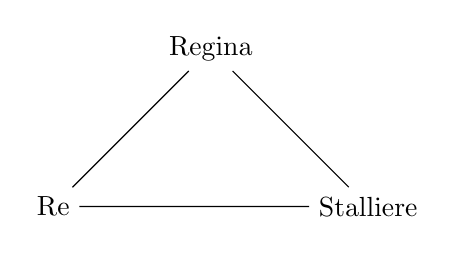
\begin{tikzpicture}
                            \node (A) at (0, 2) {Regina};
                            \node (B) at (-2, 0) {Re};
                            \node (C) at (2, 0) {Stalliere};
                            \draw (A) -- (B) -- (C) -- (A);
                        \end{tikzpicture}
                    \end{center}
                \item La donna cantata è sempre messa socialmente al vertice più alto;
                \item Amore unidirezionale che, pur non corrisposto, nobilita chi lo prova;
                \item Più la speranza diminuisce e più il desiderio cresce, il quale,
                    diventando insostenibile, porterebbe al suicidio di chi lo prova pur
                    di non soffrire più di desiderio;
                \item Lo stalliere si innamora con animo nobile;
                \item Il re e lo stalliere si trovano allo stesso piano sia sull'ambito
                    dell'ingegno, sia sul piano erotico, nonostante socialmente siano opposti;
            \end{subenumerate}
        \end{subenumerate}
    \item Sistema di valori:
        \begin{subenumerate}
            \item Nobiltà d'animo vs. ingegno:
                \begin{subenumerate}
                    \item La nobiltà d'animo è un valore cavalleresco, rappresentato dal re
                        e dalla regina;
                    \item L'ingegno è un valore borghese, rappresentato dallo stalliere, che
                        sovverte la sua condizione sociale attraverso l'astuzia;
                \end{subenumerate}
            \item Tutti e tre i personaggi guadagno da questa storia:
                \begin{subenumerate}
                    \item Lo stalliere e la regina hanno avuto una notte indimenticabile;
                    \item Il re ha convinto la regina che lui sia in grado di saperla
                        soddisfare;
                \end{subenumerate}
            \item La novella mette in luce la possibilità di sovvertire le gerarchie sociali
                attraverso l'intelligenza e l'inganno, ponendo così una tensione tra i due
                temi della nobiltà e dell'ingegno che riflette i cambiamenti sociali
                dell'epoca, con l'emergere della borghesia e dei nuovi valori legati
                all'abilità personale.
        \end{subenumerate}
\end{enumerate}

\newpage
\subsubsection{IV, 5 (Lisabetta da Messina)}
\begin{enumerate}
    \item Struttura:
        \begin{subenumerate}
            \item Premessa [§3]: Parte della cornice. Parla Filomena, la quale,
                riallacciandosi alla novella precedente di Elissa, premette che quella che
                racconterà lei non sarà una novella che tratterà di ``genti di sì alta
                condizione'', ma ciononostante non sarà meno dolorosa di quella di Elissa.
            \item Antefatto [§§4-5]:
                \begin{subenumerate}
                    \item Filomena inizia a narrare di cosa tratterà la storia;
                    \item Parla di tre fratelli mercanti a Messina, arricchiti con i soldi
                        dell'eredità del padre, con la loro sorella Lisabetta, non ancora
                        maritata;
                    \item Introduce il garzone pisano Lorenzo, che iniziò a piacere a
                        Lisabetta e, con amore corrisposto, erano diventati inseparabili
                        in anima e corpo;
                \end{subenumerate}
            \item Svolgimento dell'azione:
                \begin{subenumerate}
                    \item Protagonisti: fratelli [§§6-23]:
                        \begin{itemize}
                            \item Scoperta della tresca [§§6-7]: i fratelli di Lisabetta
                                scoprono la relazione segreta tra lei e Lorenzo;
                            \item Omicidio [§§8-9]: i fratelli uccidono Lorenzo per
                                salvaguardare l'onore della famiglia;
                            \item Domande di Lisabetta [§§10-11]: Lisabetta chiede ai suoi
                                fratelli di Lorenzo, ma riceve risposte evasive;
                        \end{itemize}
                    \item Protagonista: Lisabetta [§§11-18]:
                        \begin{itemize}
                            \item Sogno [§§12-13]: Lisabetta sogna Lorenzo che le rivela il
                                luogo della sua sepoltura;
                            \item Scoperta del cadavere e recupero della testa [§§14-16]:
                                Lisabetta si reca nel luogo indicato nel sogno, scava e
                                trova il corpo di Lorenzo, prendendo con sé la sua testa;
                            \item Culto per il vaso [§§17-18]: Lisabetta pianta la testa
                                di Lorenzo in un vaso di basilico, che cura con devozione;
                        \end{itemize}
                    \item Protagonisti: fratelli [§§19-22]:
                        \begin{itemize}
                            \item Sottrazione del vaso: i fratelli, sospettosi del
                                comportamento di Lisabetta, le sottraggono il vaso di
                                basilico e scoprono la testa di Lorenzo;
                        \end{itemize}
                    \item Protagonista: Lisabetta [§23]:
                        \begin{itemize}
                            \item Morte: Lisabetta muore di dolore, dopo aver perso sia
                                Lorenzo sia il vaso contenente la sua testa;
                        \end{itemize}
                \end{subenumerate}
            \item Origine della novella [§§23-24]: la storia di Lisabetta di Messina è un
                racconto popolare, narrato e cantato;
        \end{subenumerate}
    \item Sistema dei personaggi:
        \begin{subenumerate}
            \item Struttura dei personaggi alternata:
                \begin{subenumerate}
                    \item Evidenzia la mancanza di scambi verbali
                    tra la sorella e i fratelli, tranne nei momenti di richiesta di
                    informazioni sulla posizione del garzone, le quali non vengono neanche
                    risposte;
                    \item Per Boccaccio, l'assenza di parole indica soggezione e timore. In
                    questo caso, Lisabetta si sente intimorita dai fratelli;
                \end{subenumerate} 
            \item I personaggi si esprimono con i fatti e non con le parole:
                \begin{subenumerate}
                    \item Fratelli (personaggi forti):
                        \begin{itemize}
                            \item Usano l'azione;
                            \item Superiori dal punto di vista patriarcali (maschi) e sociali
                                (mercanti, più importanti di garzoni e fanti);
                            \item Subordinano tutto in funzione degli affari e alla loro
                                reputazione da mercanti, ragionano su costi e benefici
                                (ragione di mercatura) [§§6,7,22];
                            {\color{gray}{\item I fratelli non sono mai nominati, privi di
                                identità individuale;
                            \item Agiscono da vigliacchi, ingannando Lorenzo, 3 contro 1,
                                colpendolo alle spalle e senza assumersi nessuna
                                responsabilità [§5];}}
                        \end{itemize}
                    \item Lisabetta (+Lorenzo, +Fante) (personaggi deboli):
                        \begin{itemize}
                            \item Espressione dei sentimenti attraverso il principato
                                [§§11,12,14,16,17,18,20,23];
                            \item Rivolge domande cariche di sentimenti ai fratelli
                                [§§10,11,13,20];
                            \item Sentimenti disinteressati e genuini, non condizionati dagli
                                affari e dal lavoro;
                            \item Personaggi condannati a una condizione di inferiorità sia
                                per ragioni di sesso sia per ceto sociale;
                        \end{itemize}
                \end{subenumerate}
            In questa novella nessuno vince, la sorella perde l'amore e muore per il dolore,
            i fratelli devono lasciare il paese e perdere tutti gli affari locali;
        \end{subenumerate}
    \item Interpretazione:
        \begin{subenumerate}
            \item Interpretazione storico-ideologica:
                \begin{itemize}
                    \item Boccaccio accusa la cecità della logica mercantile del guadagno,
                        la quale non guarda in faccia a nessuno se non agli affari,
                        colpevolizzando i fratelli per la morte della sorella per presalvare
                        i loro affari;
                    \item Lorenzo e Lisabetta non hanno un monumento del loro amore. Esso
                        viene celebrato e ricordato solo a parole e nelle canzoni [§24],
                        rendendo Lisabetta una persona sconfitta;
                    \item Confronto con \underline{Lo stalliere del re Agilulf}: mentre lo
                        stalliere dopo essersi beffato del re riesce a porsi un limite,
                        i fratelli di Lisabetta non si pongono nessun limite, arrivando
                        addirittura a compiere un omicidio e a fuggire anonimamente;
                \end{itemize}
            \item Interpretazione psicoanalitica:
                \begin{itemize}
                    \item In questa novella è più importante il linguaggio non verbale
                        piuttosto di ciò che non viene detto;
                    \item Personaggi forti e deboli:
                        \begin{itemize}
                            \item  I tre fratelli non sono in grado di: amare, comunicare,
                            fare (non hanno intraprendenza: se Lorenzo non ci fosse stato,
                            loro non avrebbero avuto le capacità di fare i loro affari) [§5];
                            \item Lisabetta è in grado di: amare, comunicare, prendere
                                iniziativa;
                            \item I fratelli sotto aspetto psicoanalitico sono personaggi
                                deboli e tristi, mentre Lisabetta e Lorenzo personaggi forti
                                e felici;
                        \end{itemize}
                    \item Sviluppo dei personaggi:
                        \begin{itemize}
                            \item I tre fratelli sono privi di identità, si conosce solo che
                                sono imparentati con Lisabetta;
                            \item I tre non sono in grado di provare le stesse emozioni della
                                sorella e questo gli causa gelosia e la non accettazione di
                                non poterle provare;
                            \item La loro vigliaccheria è confermata dalla loro maleducazione
                                nelle interazioni con la sorella e con Lorenzo, che è stato
                                ucciso con l'inganno;
                            \item Colpa e sottomissione:
                                \begin{itemize}
                                    \item Lisabetta interiorizza la colpa e accetta la
                                        violenza verbale come giusta;
                                    \item Nel sogno di Lisabetta, le accuse del garzone non
                                        sono verso i fratelli ma verso di lei. Accuse
                                        chiaramente sviluppate nella sua mente e mai dette
                                        da Lorenzo, poiché lei si crede responsabile della
                                        sua morte;
                                \end{itemize}
                        \end{itemize}
                    \item Metafora materna: inizia la distorsione della realtà e la pazzia
                        di Lisabetta:
                        \begin{itemize}
                            \item La scena dell'amputazione della testa è metaforicamente
                                legata alla scena di un parto, come se la testa fosse un
                                figlio messo in un panno e dato ``in grembo'' alla serva
                                [§15];
                            \item La testa di Lorenzo diventa un simbolo di
                                amore materno e cura, il basilico rappresenta la crescita e
                                la fertilità, che Lisabetta vede crescere rigogliosa proprio
                                come una madre vede crescere un proprio figlio [§19];
                            \item La descrizione della pianta ``divenne bellissimo e 
                                odorifero molto'' [§19] è scritta molto similmente alla
                                descrizione di Lorenzo ``esendo assai bello della persona e
                                leggiadro molto'' [§X].
                        \end{itemize}
                \end{itemize}
        \end{subenumerate}
\end{enumerate}

\newpage
\subsubsection{V, 8 (Nastagio degli Onesti)}
\begin{itemize}
    \item \textbf{Rubrica:} ``Nastagio degli Onesti, amando una de’Traversari, spende le sue
        ricchezze senza essere amato. Vassene, pregato da’ suoi, a Chiassi; quivi vede
        cacciare ad un cavaliere una giovane e ucciderla e divorarla da due cani. Invita i
        parenti suoi e quella donna amata da lui ad un desinare, la quale vede questa
        medesima giovane sbranare; e temendo di simile avvenimento prende per marito
        Nastagio.'';
    \item \textbf{Tema:} amori che hanno lieto esito;
    \item \textbf{Paragrafi:}
        \begin{enumerate}
            \item Rubrica;
            \item Cornice;
            \item Inizia il discorso della novellatrice;
            \item Inizio della storia;
        \end{enumerate}
\end{itemize}
\begin{enumerate}
    \item Personaggi:
        \begin{subenumerate}
            \item Nastagio degli Onesti: nobile, ricco, giovane e orfano di padre e zio. Ama
                disperatamente una donna fino a desiderare il suicidio e spendere ingenti
                somme di denaro per lei senza ottenere nulla in cambio, cosa che lo rovina
                [§§4,7-9];
            \item Donna amata: figlia di Paolo Traversaro, nobile, sgarbata e crudele. È
                sdegnosa nei confronti di Nastagio, consapevole della propria bellezza e
                nobiltà [§§5-6];
            \item Guido degli Anastagi: cavaliere che si suicida per amore, la cui storia
                parallela a quella di Nastagio serve da monito;
        \end{subenumerate}
    \item I due racconti: la novella interseca le storie di Nastagio e di Guido:
        \begin{subenumerate}
            \item Identità: la storia di Nastagio è identica a quella di Guido:
                \begin{itemize}
                    \item Nomi simili (Nastagio // Guido degli Anastagi);
                    \item Sono entrambi di Ravenna;
                    \item Amano entrambi senza essere ricambiati;
                    \item Le donne amate sono anonime, non hanno un nome;
                    \item La donna di Nastagio è ``cruda e selvaggia'' [§6], mentre quella
                        di Guido è di una ``fierezza e crudeltà'' [§21];
                    \item Nastagio pensa al suicidio [§7], Guido di fatto si suicida [§21];
                    \item Nastagio si sforza ad odiare l'amata [§6], Guido la odia e la
                        uccide ripetutamente [§26];
                    \item L'amata è indifferente all'amore di Nastagio [§6], l'amata è
                        indifferente all'amore di Guido e oltretutto ne gode della sua morte
                        [§22];
                \end{itemize}
            \item Sviluppo possibile:
                \begin{subenumerate}
                    \item Nastagio vede nella storia di Guido un possibile sviluppo futuro
                        della sua propria storia;
                    \item Aguzza l'ingegno per cambiare il corso degli eventi della sua vita;
                \end{subenumerate}
        \end{subenumerate}
    \item La caccia infernale:
        \begin{subenumerate}
            \item Ogni venerdì, Guido insegue la donna attraverso il bosco, montando un
                cavallo nero e accompagnato da due feroci mastini;
            \item La donna, nuda e terrorizzata, cerca di scappare ma viene sempre raggiunta
                da Guido;
            \item Guido la cattura, la uccide con una spada e le strappa il cuore, gettandola
                ai cani;
            \item Questo ciclo si ripete eternamente come punizione per entrambi:
                \begin{itemize}
                    \item Punizione a Guido per essersi suicidato;
                    \item Punizione per l'amata di Guido che, crudelmente, ha goduto della
                        sua morte;
                \end{itemize}
        \end{subenumerate}
    \item La parodia: è il rovesciamento di un'opera artistica o di un tema;
        \begin{subenumerate}
            \item La novella è una parodia del genere exemplum, un racconto con finalità
                morale e didascalisca;
            \item Capovolgimento del dogma religioso:
                \begin{subenumerate}
                    \item Secondo il dogma religioso, le persone non devono concedersi a
                        tentazioni amorevoli e sessuali personali, dunque esorta a respingere
                        ogni lusinga come norma morale da seguire. Di fatto, la novella
                        capovolge questa norma morale, poiché desistere alle tentazioni è
                        immorale, rendendo corretto il lasciarsi al piacere;
                    \item Il fatto di non ricambiare l'amore in questa novella è un peccato
                        religioso;
                    \item [§30] La crudeltà va vendicata e la pietà è degna di lode, come
                        spiegato da Filomena; 
                    \item [§41] La visione della punizione eterna spinge l'amata di Nastagio a
                        cambiare repentinamente atteggiamento e a sposarlo;
                    \item [§44] Tutte le donne di Ravenna iniziano a concedersi ai loro
                        corteggiatori temendo la stessa punizione dell'amata di Guido;
                \end{subenumerate}
        \end{subenumerate}
    \item L'ingegno di Nastagio:
        \begin{subenumerate}
            \item Nastagio sfrutta a suo vantaggio la situazione vista nella foresta:
                \begin{itemize}
                    \item È furbo, ha una buona capacità di osservazione e di usare a suo
                        vantaggio gli eventi che accadono attorno a lui;
                    \item È buono d'animo, di fatto non costringe nessuno dei personaggi a
                        fare qualcosa e non li inganna;
                    \item Utilizza la visione della caccia infernale per impaurire l'amata e
                        le altre donne e a cambiare visione del rifiuto dell'amore;
                    \item Nastagio vede la proiezione della sua storia in quella di Guido e
                        cambia il corso degli eventi, così da ottenere un esito diverso [§32];
                \end{itemize}
        \end{subenumerate}
    \item L'aldilà:
        \begin{subenumerate}
            \item Capovolgimento dei temi danteschi: il Decameron è il riversamento della
                Commedia di Dante:
                    \begin{itemize}
                        \item La novella rappresenta l'inferno sulla Terra;
                        \item Boccaccio sfrutta l'oltretomba come \underline{vantaggio} per la
                            vita terrena;
                    \end{itemize}
        \end{subenumerate}
    \item Le fonti della novella: Boccaccio non inventa tutta la novella ma si ispira da
        vari testi già esistenti:
        \begin{subenumerate}
            \item Ovidio, \underline{Metamorfosi}:
                \begin{itemize}
                    \item Vertunno ama Pompona, ma lei lo respinge. Per conquistarla, Vertunno
                        si traveste da vecchia e racconta a Pompona di una donna che,
                        continuando a respingere i corteggiamenti, viene trasformata in pietra
                        per punizione. Con questo inganno, Pompona converte il suo odio in
                        amore verso Vertunno;
                \end{itemize}
            \item Andrea Cappellano, \underline{De Amore}:
                \begin{itemize}
                    \item Trattato d'amore che spiega cos'è l'amore e le strategie d'amore,
                        il quale presenta al suo interno una storia simile a questa;
                \end{itemize}
            \item Dante, \underline{Commedia}:
                \begin{itemize}
                    \item [\underline{Purgatorio}, Canto XIV] Le famiglie Onesti e Anastagi di
                        Ravenna sono due famiglie che vengono citate insieme a Dante.\\
                        La novella è una rappresentazione Dantesca, la quale comprende la legge
                        del contrappasso, il sistema di punizioni, la pena a termine e la
                        presenza di un Regno ultraterreno dopo la vita terrena;
                    \item [\underline{Inferno}, Canto XIII] Parla di due scialacquatori, uno
                        dei quali ha dato fuoco alla propria casa solo per il gusto di vederla
                        bruciale. I due, graffiati, corrono per una selva finché, inciampando,
                        non vengono sbranati da un branco di cani in eterno.
                \end{itemize}
            \item Passavanti, \underline{Il Carbonaio di Niversa}:
                \begin{itemize}
                    \item Il Carbonaio assiste alla caccia infernale di un cavaliere su un
                        cavallo nero che insegue una donna nuda che, raggiunta, viene presa
                        per i capelli, trapassata con un coltello e gettata nella fossa dei
                        carboni ardenti, quindi la carica sul cavallo e se ne torna via al 
                        galoppo;
                    \item Il cavaliere gli rivela che la condizione di cacciatore e preda gli
                        spetta poiché la donna fu sua amante ma lei lo uccise e così, come
                        l'amore dell'uomo ardeva nel suo cuore, la donna è condannata ad
                        ardere nella fossa dei carboni;
                \end{itemize}
        \end{subenumerate}
    \item Significato morale:
        \begin{subenumerate}
            \item Boccaccio critica la crudeltà e l'indifferenza, suggerendo che la durezza di
                cuore e il rigiuto possano essere peccati tanto gravi quanto la lussuria. La
                novella serve dunque a denunciare l'ipocrisia e la mancanza di pietà.
        \end{subenumerate}
\end{enumerate}

\newpage
\subsubsection{VI, 10 (Frate Cipolla)}
\begin{enumerate}
    \item Struttura:
        \begin{subenumerate}
            \item \textbf{Narratore:} Dioneo, il più bravo nello scrivere le novelle;
            \item \textbf{Tema:} cavarsi d'impiccio con l'uso della parola;
            \item \textbf{Rubrica:} ``Frate Cipolla promette a certi contadini di mostrar loro
                la penna dell'agnolo Gabriello; in luogo della quale trovando carboni, quegli
                dice esser di quegli che arrostirono san Lorenzo'';
            \item La novella non è divisibile in capitoli, poiché nel testo non è presente un
                punto che determina un cambiamento drastico. Fin da subito sappiamo che frate
                Cipolla, nonostante non sia un intellettuale, ha un'eccellente abilità nel
                parlato, qualità che si riconferma a fine novella. Il protagonista si affida
                ciecamente al suo fante, del quale sappiamo ancora le sue caratteristiche sin
                da subito, ossia che ha un aspetto fisico disustoso e che ha poco intelletto;
        \end{subenumerate}
    \item Personaggi:
        \begin{subenumerate}
            \item Frate Cipolla: protagonista, è un frate antoniano dai capelli rossi, piccolo
                di statura e abile imbroglione. È noto per la sua eccellente abilità oratoria,
                che gli permette di convincere e ingannare il pubblico con destrezza [§7];
            \item Guccio Imbratta:
                \begin{itemize}
                    \item Servo di Frate Cipolla, descritto come sudicio, stupido e pieno di
                        peccati [§15]. Ha nove cose: ``egli è tardo, sugliardo e bugiardo;
                        negligente, disubbidiente e maldicente; trascurato, smemorato e
                        scostumato'' [§17];
                    \item La prova testuale delle nove cose si ha durante la scena di Guccio
                        che, uscendo di testa per un misero paio di poppe, si distrae e lascia
                        incustodita la cassetta contenente la penna dell'Arcangelo Gabriele
                        [§§20-25];
                \end{itemize}
            \item Serva Nuta: ``grassa e grossa e piccola e mal fatta, con un paio di poppe che
                parevan due ceston da letame e con un viso che parea de'Baronci, tutta sudata,
                unta e affumicata, non altrimenti che si gitti l'avoltoio alla carogna'' [§21];
            \item Giovanni e Biagio: sono amici di Frate Cipolla, intelligenti e furbi, che
                decidono di sostituire la penna con dei carboni per beffare il Frate e metterlo
                alla prova sulla sua abilità oratorio e d'ingegno;
        \end{subenumerate}
    \item Elementi comici:
        \begin{subenumerate}
            \item Discorso di Guccio Imbratta [§22]:
                \begin{itemize}
                    \item Guccio cerca di sedurre Nuta con un discorso breve e inventato,
                        puntando su menzogne e sul fatto che lui fosse di buona famiglia,
                        cercando di imitiare l'ingegno oratorio di Frate Cipolla, fallendo
                        miseramente nel suo intento, a contrario di Cipolla;
                \end{itemize}
            \item Discorso di Frate Cipolla:
                \begin{itemize}
                    \item Riesce a convincere l'intera popolazione di Certaldo con un discorso
                        lungo e articolato. [§37] Apre il discorso dicendo di essere stato
                        nel luogo dove sorge il sole, frase gonfiata che indicativamente
                        può rappresentare qualsiasi posto sulla Terra. Inoltre, parla di grandi
                        banalità ma con un registro epico e inventando parole esotiche, facendo
                        immaginare al popolo di aver vissuto eventi miracolosi;
                \end{itemize}
        \end{subenumerate}
    \item Pubblico: Dioneo, narratore della novella, rivela agli ascoltatori della novella le
        dinamiche nascoste, aggiungendo un livello di ironia e complicità con gli altri nove:
        \begin{subenumerate}
            \item Certaldo: il principale ascoltatore di Frate Cipolla è l'intera popolazione
                di Certaldo, inclusi Giovanni e Biagio, che conoscono la verità sullo scambio
                della penna;
            \item Giovanni e Biagio insieme formano un pubblico nascosto che, tra tutte le
                altre persone, sono gli unici che si divertono a crepapelle poiché sanno di
                essere stati loro a sostituire la penna con il carbone.
            \item Dioneo: l'informazione del pubblico nascosto si protrae agli ascoltatori
                della novella, i quali si sentono parlare di Firenze come un luogo miracoloso.
                Tutto questo poi si protrae ai lettori, i quali sanno già dalla rubrica che
                Frate Cipolla sarà in grado di cavarsi d'impiccio grazie all'uso della parola;
        \end{subenumerate}
    \item La polemica religiosa:
        \begin{subenumerate}
            \item Frate Cipolla è un ingannatore che sfrutta la credulità popolare per ottenere
                donazioni per la chiesa;
            \item Boccaccio non lo accusa direttamente di essere un imbroglione, ma ne elogia
                l'abilità oratoria e la capacità di cavarsi d'impiccio per poi avere un
                resoconto materiale;
            \item La novella critica indirettamente il commercio delle reliquie e l'ipocrisia
                della classe ecclesiastica, senza esprimere giudizi morali e focalizzandosi
                più sugli eventi terreni che sulle conseguenze nell'aldilà. 
        \end{subenumerate}
\end{enumerate}

\newpage
\subsubsection{VII, 1 (Gianni Lotteringhi e la ``fantasima'')}
\begin{enumerate}
    \item Struttura:
        \begin{subenumerate}
            \item \textbf{Narratrice:} Emilia;
            \item \textbf{Tema:} beffe delle mogli ai mariti;
            \item \textbf{Luogo:} Firente, contrada di San Brancazio;
        \end{subenumerate}
    \item Personaggi:
        \begin{subenumerate}
            \item Gianni Lotteringhi: è uno stamaiuolo (lavoratore e venditore di stame),
                semplice e devoto al lavoro. È il capitano della confraternita dei laudesi di
                Santa Maria Novella. È bigotto, chiuso, supertizioso e donava alla chiesa per
                venir benedetto dai Frati. Aveva una donna bellissima per moglie [§4];
            \item Tessa: bellissima e vaga per moglie, savia e avveduta, figlia di Mannuccio
                dalla Cuculia. È consapevole della semplicità del marito, si innamora di
                Federigo di Neri Pegoletti e organizza incontri con lui nella casa estiva a
                Camerata. Tessa inganna il marito con astuzia, sfruttando la sua superstizione
                [§6];
            \item Federigo di Neri Pegoletti: bello e fresco giovane, amante di Tessa.
                Rappresenta i valori ``nuovi'' e contrastanti a quelli di Gianni [§6];
        \end{subenumerate}
    \item Triangolo amoroso: la donna cantata è posta al vertice, mentre i due uomini sono
        posti alla base del triangolo.:
            \begin{center}
                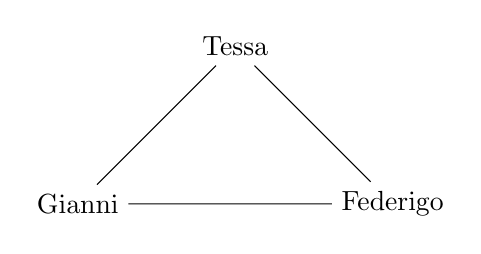
\begin{tikzpicture}
                    \node (A) at (0, 2) {Tessa};
                    \node (B) at (-2, 0) {Gianni};
                    \node (C) at (2, 0) {Federigo};
                    \draw (A) -- (B) -- (C) -- (A);
                \end{tikzpicture}
            \end{center}
        I due si trovano ai vertici opposti poiché:
            \begin{itemize}
                \item Cibo: Tessa prepara a Gianni cibo semplice, mentre a Federigo cucina
                    capponi, uova e vino [§§12,13];
                \item Sesso: Federigo ha una relazione intima con Tessa, mentre Gianni è
                    sessualmente inattivo [§§8,20];
                \item Preghiere: Gianni prega sinceramente, mentre Federigo le utilizza in modo
                    allusivo ed erotico [§§20,8];
            \end{itemize}
    \item La beffa:
        \begin{subenumerate}
            \item Architettura: la beffa è ingegnosamente architettata da Tessa, che
                sfrutta la superstizione del marito Gianni per continuare la sua relazione
                con Federigo. Usa il teschio come segnale per comunicare con l'amante e
                crea una storia di fantasmi per distogliere l'attenzione del marito;
            \item Esecuzione: quando Gianni torna a casa inaspettatamente, Tessa
                improvvisa una spiegazione per il rumore della porta, coinvolgendolo in una
                filastrocca per ``scacciare il fantasma'' che la molestava da alcune sere.
                La filastrocca è un metodo per poter comunicare con Federigo, nella quale
                infatti dice che il marito è a casa e dà indicazioni su dove trovare il
                cibo preparato. Federigo, sentendo la filastrocca, ride di gusto e se ne
                va.
            \item Il ricordo: Tessa e Federico scherzeranno le sere future di questo
                imprevisto basato sull'ingenuità del marito;
        \end{subenumerate}
    \item Sistema dei valori:
        \begin{subenumerate}
            \item Boccaccio non critica direttamente Gianni, bensì ne ridicolizza la
                superstizione e l'ingenuità, mentre esalta l'astuzia e l'intelligenza di Tessa;
            \item La morale della novella, detta da Emilia, è rivolta alle donne, la quale
                dice di prendere spunto dall'ingenuità degli uomini per trovare una
                scappatoia e divertimento.
        \end{subenumerate}
\end{enumerate}

\newpage
\section{Niccolò Machiavelli}

\begin{enumerate}
    \item Niccolò Machiavelli è stato un influente pensatore, diplomatico e scrittore fiorentino 1469-1527
    \item Nato a Firenze in una famiglia di modeste origini,
    \item educazione umanistica e divenne coinvolto nella politica fiorentina
\end{enumerate}

\subsection{Modelli di comportamento: il trattato}
\subsubsection{Lettera al Vettori}

\begin{enumerate}
    \item 10 dicembre 1513 indirzzata a Francesco Vettori, una delle due opere molto famosa
    \item discute degli eventi politici dell’epoca, in particolare il suo recente licenziamento da parte dei Medici dopo la caduta della Repubblica di Firenze.
    \item è delusione per essere stato escluso dalla vita
    politica e riflette sulle difficoltà e le instabilità della politica italiana.
    \item Gli condivide le sue preoccupazioni
    sulla situazione politica del tempo e sulla necessità di un principe forte e capace per riportare l’ordine e
    la stabilità nella regione
    \item Discute anche della natura umana sottolineando la necessità per un
    governante di adattarsi alle circostanze e di essere disposto a prendere decisioni impopolari per il bene
    comune
    \item L’esilio del 1512 denota uno spartiacque.
    \item prima incontrava il re di Francia, mentre ora le
    sue giornate sono monotone e non sa cosa fare
    \item da un certo punto Machiavelli comincia a tenere
    il proprio cervello vivo studiando (leggendo): questo è il senso della sua vita, rialzando la sua scrittura.
    \item I luoghi della sua giornata sono essenzialmente tre:
    \begin{itemize}
        \item \textbf{naturali} (luoghi aperti, bosco, etc.).
            Questi luoghi sono rappresentanti delle occupazioni pratiche (caccia di uccelli, commercio, taglio legna etc.);
        \item \textbf{la strada} (luogo di riflessione e di incontro con le persone dei paesi vicini);
        \item \textbf{osteria, scrittoio} (luoghi chiusi). Questi due posti sono quasi antitetici per la loro natura.
    \end{itemize}
    \item Un ragionamento analogo può essere svolgo circa i tempi della sua giornata:
    \begin{itemize}
        \item \textbf{mattino} (occupazioni pratiche);
        \item \textbf{pomeriggio} (vita sociale);
        \item \textbf{sera e di notte} (tempo per sè, tempo dello studio).
    \end{itemize}
    \item Nella lettera vi è una incongruenza. Vengono indicati solamente i principati come argomento, quando il libro finale sarà
    più vasto. Nella lettera sembra implicare che il libro sia finito. Il libro è quindi finito o no?
    \item Inoltre dice che la dedica sarà a Giulinao de' Medici, ma in realtà lo sarà a Lorenzo il giovane.
    \item Prima descrive il libro come un ghiribizzo, quasi come un piccolo gioco, ma successivamente dice
    che può essere usato da un principe nuovo.
    \item Il dubbio dilemmatico è quello di consegnare il libro. E se darlo, darglielo personalmente o per altri
    mezzi? La lettera è quindi piena di dissirio e molto problematica.
\end{enumerate}

\newpage
\subsection{Il Principe}
\subsubsection{Dedica}

\begin{enumerate}
    \item \textbf{Introduzione alla dedica}
    \begin{enumerate}[label*=\arabic*.]
        \item Machiavelli cerca di entrare nelle grazie di un sovrano.
        \item Offre qualcosa di prezioso o gradito: \textit{la cognizione delle azioni degli uomini grandi}.
        \begin{itemize}
            \item La parola \textit{grande} indica persone di potere, senza connotazione morale.
        \end{itemize}
        \item Conoscenza acquisita da:
        \begin{itemize}
            \item Lunga esperienza delle cose moderne.
            \item Lettura dei testi antichi.
        \end{itemize}
        \item Conoscenza offerta tramite un piccolo volume: \textit{Il Principe}.
        \item Vantaggio del dono: sintesi di migliaia di pagine lette e quindici anni di esperienza.
    \end{enumerate}

    \item \textbf{Topos della modestia}
    \begin{enumerate}[label*=\arabic*.]
        \item Opposizione fra modestia e orgoglio nei testi di Machiavelli.
        \item Machiavelli minimizza l'importanza delle sue opere, pur riconoscendone la grandezza e importanza.
    \end{enumerate}

    \item \textbf{Descrizione della forma del libro}
    \begin{enumerate}[label*=\arabic*.]
        \item Esteticamente poco attraente.
        \item Machiavelli vuole che il testo venga apprezzato solo per il suo contenuto.
        \item Assenza di ornamenti per evitare che il libro venga apprezzato per altro che non sia il contenuto.
    \end{enumerate}

    \item \textbf{Giustificazione dell'autore}
    \begin{enumerate}[label*=\arabic*.]
        \item Machiavelli non vuole essere visto come presuntuoso.
        \item Paragone con pittori/cartografi:
        \begin{quote}
            \itshape
            Nè voglio sia riputata presunzione, se uno uomo di basso ed infimo stato ardisce discorrere e regolare i governi de' Principi; perchè così come coloro che disegnano i paesi, si pongono bassi nel piano a considerare la natura de' monti e de' luoghi alti, e per considerare quella de' bassi si pongono alti sopra i monti; similmente, a cognoscer bene la natura de' popoli bisogna esser Principe, ed a cognoscer bene quella de' Principi conviene essere popolare.
        \end{quote}
        \item Per parlare del popolo bisogna essere principi, per parlare dei principi bisogna essere del popolo.
        \item Questa è la motivazione di Machiavelli per scrivere il principato.
    \end{enumerate}

    \item \textbf{Conclusione della dedica}
    \begin{enumerate}[label*=\arabic*.]
        \item Machiavelli si rivolge a Lorenzo de' Medici.
        \item Gli augura il meglio nel suo potere.
        \item Sottolinea la propria posizione sfortunata.
    \end{enumerate}
\end{enumerate}

\newpage
\subsubsection{Capitolo I}

\begin{enumerate}
    \item \textbf{Introduzione}
    \begin{enumerate}[label*=\arabic*.]
        \item Citazione iniziale:
        \begin{quote}
            \itshape
            Tutti gli Stati, tutti i dominii che hanno avuto, e hanno imperio sopra gli uomini, sono stati e sono o Repubbliche o Principati.
        \end{quote}
        \item Differenza tra repubblica e principato.
        \begin{itemize}
            \item Repubblica: più democratica e partecipativa.
            \item Principato: incentrato su una singola persona o gruppo di persone. XXX
        \end{itemize}
    \end{enumerate}

    \item \textbf{Tipologie di Principati}
    \begin{enumerate}[label*=\arabic*.]
        \item Principati nuovi e ereditari.
        \begin{itemize}
            \item Principati nuovi:
            \begin{itemize}
                \item Completamente nuovi (es. Milano a Francesco Sforza).
                \item Aggiunti ad una conquista (es. Regno di Napoli al Re di Spagna).
            \end{itemize}
            \item Principati ereditari: governati da una lunga discendenza.
        \end{itemize}
        \item Citazione di esempi storici per i principati nuovi aggiunti a una conquista.
    \end{enumerate}

    \item \textbf{Termine tecnico: \textit{acquista}}
    \begin{enumerate}[label*=\arabic*.]
        \item Significato specifico di \textit{acquista} in Machiavelli: conquistare.
    \end{enumerate}

    \item \textbf{Metodi di conquista dei popoli}
    \begin{enumerate}[label*=\arabic*.]
        \item Popoli abituati alla libertà vs. popoli abituati al dominio di un principe.
        \item Conquista tramite:
        \begin{itemize}
            \item Armi d'altri (mercenari, prestate o comprate).
            \item Proprio esercito di milizia.
        \end{itemize}
    \end{enumerate}

    \item \textbf{Fortuna e virtù nella conquista}
    \begin{enumerate}[label*=\arabic*.]
        \item Conquista per fortuna: ciò che sfugge al calcolo umano.
        \item Conquista per virtù:
        \begin{itemize}
            \item Capacità tecniche del principe.
            \item Virtù come abilità, non connotazione morale.
        \end{itemize}
        \item Il principe virtuoso possiede capacità tecniche, non necessariamente qualità morali come saggezza e onestà.
    \end{enumerate}
\end{enumerate}

\newpage
\subsubsection{Capitolo VI}

\begin{enumerate}
    \item \textbf{Introduzione}
    \begin{enumerate}[label*=\arabic*.]
        \item Citazione iniziale:
        \begin{quote}
            \itshape
            De' Principati nuovi, che con le proprie armi e virtù si acquistano.
        \end{quote}
        \item Concetto di imitazione:
        \begin{itemize}
            \item Importanza di ispirarsi a modelli altissimi.
            \item Analogía dell'arciere: mirare più in alto per raggiungere il bersaglio.
        \end{itemize}
    \end{enumerate}

    \item \textbf{Modelli da imitare}
    \begin{enumerate}[label*=\arabic*.]
        \item Personaggi indicati da Machiavelli:
        \begin{itemize}
            \item \textit{Moisè}: legislatore e fondatore del popolo ebraico di Israele.
            \item \textit{Ciro II}: fondatore della monarchia di Persia.
            \item \textit{Romolo}: personaggio legato al mito della fondazione di Roma.
            \item \textit{Teseo}: re mitologico di Atene.
        \end{itemize}
        \item Caratteristiche comuni:
        \begin{itemize}
            \item Fondatori di regni o repubbliche.
            \item Successo dovuto alle proprie capacità, non alla fortuna.
            \item Difficile riconoscimento iniziale e nessuna agevolazione.
        \end{itemize}
        \item Distinzione di Machiavelli:
        \begin{itemize}
            \item Unico personaggio realmente esistito: Ciro.
            \item Moisè aveva il privilegio di parlare con Dio.
        \end{itemize}
    \end{enumerate}

    \item \textbf{Virtù e fortuna nella conquista}
    \begin{enumerate}
        \item Virtù:
        \begin{itemize}
            \item Fatica per raggiungere la carica, ma mantenimento semplice.
        \end{itemize}
        \item Fortuna:
        \begin{itemize}
            \item Guadagno della carica semplice, ma fatica nel mantenerla.
        \end{itemize}
        \item Occasione come elemento intermedio tra virtù e fortuna.
        \begin{itemize}
            \item La virtù permette di riconoscere e sfruttare l'occasione.
            \item Minima fortuna necessaria, ma grande virtù può compensare l'assenza di fortuna.
        \end{itemize}
    \end{enumerate}

    \item \textbf{Esempi di fortuna e virtù nei modelli}
    \begin{itemize}
        \item \textit{Moisè}: trovò il popolo di Israele schiavo e oppresso in Egitto.
        \item \textit{Ciro}: trovò i Persiani malcontenti.
        \item \textit{Romolo}: fu allontanato dal suo paese natale.
        \item \textit{Teseo}: trovò una popolazione dispersa e la riunì.
    \end{itemize}

    \item \textbf{Sostenitori del vecchio e nuovo regime}
    \begin{enumerate}[label*=\arabic*.]
        \item Maggiore aggressività dei sostenitori del vecchio regime, che lottano per certezze.
        \item Tiepidezza dei sostenitori del nuovo regime, che lottano per un'idea.
        \item Necessità di convinzioni forti per una lotta efficace.
    \end{enumerate}

    \item \textbf{Autosufficienza del principe}
    \begin{enumerate}[label*=\arabic*.]
        \item Autosufficienza essenziale per il successo del principe.
        \item Necessità di forza armata per mantenere il potere.
    \end{enumerate}

    \item \textbf{Convinzioni del popolo}
    \begin{enumerate}[label*=\arabic*.]
        \item Facilità di convincere il popolo, difficoltà di fargli cambiare idea.
        \item Uso delle armi per cambiare le convinzioni radicate.
    \end{enumerate}

    \item \textbf{Esempio di Ierone (Gerone) Siracusano}
    \begin{enumerate}[label*=\arabic*.]
        \item Diventò principe di Siracusa senza esperienza di potere, con l'occasione data dalla fortuna.
        \item Eliminò il vecchio esercito per crearne uno proprio e fedele.
        \item Cambiò alleanze e governò facilmente su fondamenta solide.
    \end{enumerate}
\end{enumerate}

\newpage
\subsubsection{Capitolo XV}

\begin{enumerate}[label*=\arabic*.]
    \item Introduzione al Capitolo XV:
    \begin{enumerate}[label*=\alph*.]
        \item Argomento principale del capitolo: il comportamento del principe verso sudditi e amici.
        \item Machiavelli inserisce il suo lavoro nella tradizione politica.
        \item Novità di Machiavelli: distacco dagli approcci tradizionali.
        \item Scopo dell'autore: utilità pratica dei principi.
        \item Utilizzo della verità effettiva anziché dell'immaginazione.
    \end{enumerate}
    
    \item Descrizione del Principe Perfetto:
    \begin{enumerate}[label*=\alph*.]
        \item Critica ai principi utopici basati sull'idealizzazione.
        \item Discrepanza tra realtà effettiva e immaginazione utopica.
        \item L'autore sostiene che il comportamento morale può portare alla perdita di potere.
        \item Descrizione delle virtù e dei vizi associati al principe.
    \end{enumerate}
    
    \item Ruolo dei Vizi:
    \begin{enumerate}[label*=\alph*.]
        \item Accettazione dei vizi se necessari per il bene dello stato.
        \item Giustificazione delle azioni basata sull'utilità politica anziché sulla morale.
        \item Passaggio dai valori assoluti ai valori relativi.
        \item Concetto di lealtà e sveltezza come termini neutri.
    \end{enumerate}
\end{enumerate}

\newpage
\subsubsection{Capitolo XVIII}

\begin{enumerate}[label*=\arabic*.]
    \item Tema principale del Capitolo XVIII:
    \begin{enumerate}[label*=\alph*.]
        \item Discussione su lealtà, slealtà e mantenimento della parola.
        \item Contrasto tra virtù ideali e realtà effettuale.
    \end{enumerate}
    
    \item Utilizzo della Forza e della Bestialità:
    \begin{enumerate}[label*=\alph*.]
        \item Il principe deve saper utilizzare sia la legge che la forza.
        \item Analogia con l'eroe greco Achille e il centauro.
        \item Sottolineatura della debolezza dell'argomentazione mitologica.
    \end{enumerate}
    
    \item Suddivisione della Forza Bestiale:
    \begin{enumerate}[label*=\alph*.]
        \item Astuzia della volpe e forza del leone.
        \item La parola data può essere infranta per motivi di convenienza o per prevenire danni.
        \item Necessità di adattare il comportamento alle circostanze.
    \end{enumerate}
    
    \item Inganno e Manipolazione:
    \begin{enumerate}[label*=\alph*.]
        \item Il principe non deve farsi notare quando inganna.
        \item Semplicità e ingenuità degli uomini che facilita la manipolazione.
        \item Importanza dell'immagine virtuosa del principe.
    \end{enumerate}
    
    \item Giudizio basato sui Risultati:
    \begin{enumerate}[label*=\alph*.]
        \item Il principe è giudicato in base ai fini che raggiunge.
        \item La popolazione mondiale è manipolabile.
    \end{enumerate}
\end{enumerate}

\newpage
\subsubsection{Capitolo XXV}

\begin{enumerate}[label*=\arabic*.]
    \item Tema principale del Capitolo XXV:
    \begin{enumerate}[label*=\alph*.]
        \item Discussione sul ruolo della fortuna nella vita dei principi.
        \item Contrapposizione tra la percezione comune della fortuna e la visione di Machiavelli.
    \end{enumerate}
    
    \item Immagine della Fortuna:
    \begin{enumerate}[label*=\alph*.]
        \item Descrizione della fortuna come un fiume in piena.
        \item Necessità di adattare il comportamento umano agli eventi della fortuna.
        \item Assenza di difese contro la fortuna in Italia.
    \end{enumerate}
    
    \item Ruolo della Virtù:
    \begin{enumerate}[label*=\alph*.]
        \item Importanza della virtù nel resistere alla fortuna.
        \item Relazione tra azioni dei principi e felicità o infelicità.
        \item Esempi di successo e fallimento in base all'adattamento alle circostanze.
    \end{enumerate}
    
    \item Approccio consigliato:
    \begin{enumerate}[label*=\alph*.]
        \item Preferenza per l'impetuosità rispetto al rispetto.
        \item Analisi della fortuna come simile a una donna, più facilmente conquistata con audacia.
        \item Vantaggio dei giovani nell'affrontare la fortuna con audacia.
    \end{enumerate}
\end{enumerate}

\newpage
\section{Ludovico Ariosto}

\subsection{Orlando furioso}

\begin{enumerate}
    \item Celebre poeta e drammaturgo italiano del Rinascimento (1474-1533)
    \item Visse principalmente a Ferrara, dove servì sotto il patronato dei duchi d'Este.
    \item Inizialmente intraprese la carriera giuridica, ma il suo vero amore era la poesia.
    \item Fu attivo anche come diplomatico e funzionario di corte, occupando diverse posizion
\end{enumerate}

\subsubsection{Canto I (ottave 1-44)}

\begin{enumerate}
    \item I due grandi temi del libro sono: \begin{subenumerate}
        \item L'amore (ispirato alla letteratura Bretone, la quale si sviluppò in Bretagna e in altre aree celtiche, principalmente
        a partire dal IX secolo in poi. Essa comprende leggende sui Celti (popoli indoeuropei) e la storia
        mitologica delle Isole britanniche e della Bretagna, in particolar modo quelle riguardanti re Artù e i
        suoi cavalieri della Tavola Rotonda.)
        \item La guerra (ispirato alla letteratura Carolingia, uno stile di scrittura creato durante la rinascita
        carolingia, che mirava a recuperare e preservare il sapere classico, avvenuta sotto il regno di Carlo
        Magno nei secoli VIII e IX.)
    \end{subenumerate}
    \item Tradizionalmente il proemio è suddiviso in tre parti: protasi, invocazione e dedica.
    \item La prima parte è la protasi cioè la dichiarazione della materia di cui parlerà il libro, in questo caso va
    dall’ottava 1 all’ottava 2 verso 4. 
    \item Poi c’è l’invocazione che occupa soltanto la seconda parte della seconda
    ottava (2.4 - 2.8).
    \item Infine, c’è la dedica che va dall’ottava 3 alla 4.
    \item \textbf{Prima ottava:} \begin{subenumerate}
        \item Vi è un doppio chiasmo (v. 1 donne, amori, cavalieri, armi e vv. 1-2 donne, amori, cortesie, cavalieri, armi, audaci imprese)
        \item Il chiasmo rappresenta il tema dell'amore e della guerra
        \item Rappresenta anche il ciclo del libro, un intrecciarsi fra idue temi come il chiasmo.
        \item La struttura dei primi due versi segue un ordine non “corretto”, il soggetto che parla è all’ultimo.
        Dunque, apparentemente l’Orlando viene scritto in maniera oggettiva, il poeta si mette in secondo piano.
        L’oggettività sta nel mettere la materia prima del narratore.
    \end{subenumerate}
    \item \textbf{Seconda ottava:} \begin{subenumerate}
        \item L'autore parlerà di una cosa che non ha mai scritto nessuno, ossia l’impazzimento di Orlando a causa
        dell’amore, lui che era così saggio.
        \item Orlando è un personaggio storico, paladino di un nobile, sotto Carlo
        Magno, ma le storie di pazzia dell’innamoramento sono inventate.
        \item Questo innamoramento è straordinario
        perché Orlando era particolarmente saggio. Anche se una persona così saggia come lui può impazzire per
        amore, da questa sorte non è al riparo nessuno. 
        \item Abbiamo la figura della lima che con il suo agire costante, erode nel tempo.
    \end{subenumerate}
    \item \textbf{Terza ottava:} \begin{subenumerate}
        \item Questi versi rappresentano un esempio di cortesia e ammirazione nei confronti del destinatario del
        canto, Ippolito d’Este, figlio di Ercole I d’Este.
        \item Il poeta esprime la sua gratitudine e il suo rispetto per
        Ippolito, riconoscendolo come un ornamento e uno splendore del suo tempo.
        \item Il tono del canto è deferente e rispettoso, e Ariosto si colloca in una posizione di umiltà di fronte al
        destinatario. 
        \item Utilizza l’immagine di sé stesso come ”umile servo” di Ippolito, sottolineando il suo desiderio
        di compiacerlo con il suo lavoro poetico
        \item Il verso finale, ”che quanto io posso dar, tutto vi dono”, sottolinea l’impegno totale del poeta nel rendere
        omaggio e onore a Ippolito, promettendo di dedicargli tutto ciò che può offrire, sia in parole che in azione.
        \item Vi è quindi una costruzione di distacco fra poeta e destinatario, un rapporto tra modestia e orgoglio. Viene
        utilizzato il registro encomiastico (scopo di lodare, elogiare).
    \end{subenumerate}
    \item \textbf{Quarta ottava:} \begin{subenumerate}
        \item Quando Ariosto parla di Ruggiero (“e de’ vostri avi illustri il ceppo vecchio.”), sta facendo riferimento
        all’antenato fondatore della casata stessa di Ippolito. 
        \item e vicende di Ruggiero sono quelle che permettono di
        elogiare il destinatario.
        \item Il penultimo verso indica uno sminuimento della posizione di Ariosto (i vostri alti
        pensieri cedano un poco per compensare i miei).
    \end{subenumerate}
    \begin{subenumerate}
        \item Orlando è stato innamorato della bella Angelica per lungo tempo.
        \item Orlando riesce a portarla in Occidente, trovando una situazione di guerra con re Carlo accampato.
        \item \textbf{Trofei infiniti:} Indica un vastissimo numero di vittorie e successi in battaglia.
        \item \textbf{Trofei immortali:} Le vittorie di Orlando sono memorabili e destinate a essere ricordate per sempre, simboli di eroismo e di valore eterno.
        \item La "bella Angelica" è un epiteto ornans.
    \end{subenumerate}
    \item \textbf{Sesta ottava:}
    \begin{subenumerate}
        \item Re Carlo si accampa per far pentire il re Marsilio (re della Spagna musulmana) e il re Agramante (re dell'Africa, musulmano) delle loro azioni contro la Francia.
        \item Orlando torna con la donna amata e si pente di essere arrivato in quel momento.
    \end{subenumerate}
    \item \textbf{Settima ottava:}
    \begin{subenumerate}
        \item Carlo Magno stesso sottrae Angelica da Orlando.
        \item Quella che aveva difeso con tanto impegno gli viene portata via dagli amici.
        \item Carlo Magno voleva "estinguere un incendio" metaforicamente, riferendosi a una pericolosa contesa d'amore.
        \item Giudizio esplicito di Ariosto sull'errore del giudizio umano.
    \end{subenumerate}
    \item \textbf{Ottava ottava:} \begin{subenumerate}
        \item In questa ottava viene spiegato la metafora dell’incendio.
        \item Il motivo è che il conte Orlando e suo
        cugino Rinaldo sono erano innamorati di Angelica.
        \item Re Carlo, temendo una riduzione dell’efficienza
        dei due guerrieri più bravi, sottrae la donna per non farli distrarre.
        \item La donna viene data a Namo, il duca di
        Bavera, per custodirla.
    \end{subenumerate}
    \item \textbf{Nona ottava:} \begin{subenumerate}
        \item La donna viene promessa a chi fra Orlando e il cugino farà più morti in questa battaglia - premio
        per chi fa più morte.
        \item Questa ottava è bipartita perché, nella sua seconda parte, in modo tutto imprevedibile,
        i cristiani (gente battezzata) perdono la battaglia e si devono ritirare. 
        \item Namo viene imprigionato e non può
        più custodire Angelica, per cui rimane sola.
        \item Qui termina l’Orlando innamorato. Dalla prossima ottava la storia è tutta un’invenzione.
    \end{subenumerate}
    \item \textbf{Decima ottava:} \begin{subenumerate}
        \item Angelica, ancora prima dell’esito della battaglia, aveva intuito che sarebbe andata male per i cristiani, e si
        era preparata a scappare. 
        \item Non perde tempo e scappa a cavallo. Incontra un cavaliere a piedi.
        \item Un tipico elemento di Ariosto è il luogo di una selva, una stretta via labirintica dove, per caso, incontra
        un cavaliere. Questo caso è il tema fondamentale di Ariosto.
    \end{subenumerate}
    \item \textbf{Undicesima ottava:} \begin{subenumerate}
        \item L’ottava è bipartita perfettamente a metà.
        \item Nella prima parte abbiamo la descrizione del cavaliere,
        mentre la seconda è la reazione di Angelica
        \item La prima parte può ancora essere suddivisa a metà, perché i
        primi due descrviono l’aspetto fisico, mentre gli altri due parlano di come il cavaliere si muovesse: più rapido
        di chi un contadino che sta partecipando ad una gara dove bisognasse inseguire un panno e prenderlo.
        \item Appena Angelica vede il cavaliero, si ferma con una rapidità maggiore di una timida pastorella che si scansa
        quando si trova un serpente in mezzo ai piedi. Angelica ha quindi una reazione terrorizzata. 
        \item Nei primi due
        versi abbiamo un chiasmo doppio fra la parte del corpo e l’arma/oggetto (Indosso, Corazza, Elmo, Testa
        e successivamente Spada, Braccio, Fianco, Scudo).
        \item La struttura dell’ottava rappresenta un chiasmo dove
        i versi 11.1-2 parlano dell’aspetto esteriore del cavaliere, mentre 11.5-6 parlano dell’aspetto esteriore della
        pastorella, e 11.3-4 è il movimento del villano, mentre 11.7-8 sono il movimento di Angelica.
        \item Vi è anche
        un altro chiasmo dove i distici parlano del movimento nei versi interni, mentre ai versi esterni parlano dei
        personaggi.
    \end{subenumerate}
    \item \textbf{12 ottava:} \begin{subenumerate}
        \item Il cavaliere era il figlio del duca Amone, Rinaldo, uno dei cugini, solo adesso viene svelato la sua
        identità. Rinaldo sta inseguendo il cavallo Baiardo che era scappato per sbaglio.
        \item Questa storia è stata
        raccontata nell’Orlando innamorato
        \item Abbiamo un’allusione al nome Angelica mediante la sembianza
        angelica, e la visione delle reti come catturato dall’amore (classiche metafore stilnovistica).
    \end{subenumerate}
    \item \textbf{13 ottava:} \begin{subenumerate}
        \item Angelica non sceglie la strada, ma lascia che il cavallo la scelga al posto suo, fino ad arrivare ad un
        fiume. Il movimento casuale viene indicato da diverse espressioni.
        \item Nell’Orlando innamorato, Angelica e Rinaldo avevano bevuto da delle fontane magiche: Angelica da quella
        che fa innamorare, per cui si era innamorata di Rinaldo, mentre Rinaldo da quella che fa odiare, per cui
        odiava Angelica. Successivamente, i due bevettero dalle fontane opposte. Il motivo per cui Angelica ha
        questa reazione è quindi perché odia e prova ribrezzo per Rinaldo.
    \end{subenumerate}
    \item \textbf{14 ottava:} \begin{subenumerate}
        \item Sulla riviera trovò Ferraù, un guerriero musulmano.
        \item Questo guerriera, pensava che si sarebbe fermato a bere
        dell’acqua e a riposare, ma dalla sua sete il suo elmo era caduto nel fiume, e non l’aveva ancora recuperato.
    \end{subenumerate}
    \item \textbf{15 ottava:} \begin{subenumerate}
        \item Il guerriero riconosce Angelica nonostante fosse pallida e terrorizzata e non avesse avuto notizie su
        di lei. Anche il guerriero è innamorato di lei. 
    \end{subenumerate}
    \item \textbf{16 ottava:} \begin{subenumerate}
        \item Il guerriere le porge tutto il suo aiuto, nonostante non avesse l’elmo.
        \item Prende la spada per difenderla
        da chiunque stesse arrivando.
        \item Più volte i due si erano già visti e si erano anche combattuti (Orlando
        innamorato).
        \item Ferraù ha questa reazione istintiva per la sua cortesia (possiede i valori cavallereschi, come
        difendere la donzella perseguitata).
    \end{subenumerate}
    \item \textbf{17 ottava:} \begin{subenumerate}
        \item L’ottava è bipartita.
        \item La prima parte è dedicata al duello (ad armi pari).
        \item I colpi che si davano, non
        solo sfondavano le piastre, ma avrebbero spezzato anche le incudini (iperbole).
        \item La seconda parte parla
        dell’esito del duello
        \item Mentre i due si stanno ammazzando, Angelica scappa con il suo cavallo.
    \end{subenumerate}
    \item \textbf{18 ottava:} \begin{subenumerate}
        \item Entrambi sono abilissimi guerrieri, e nessuno dei due riesce a sopraffare l’altro.
        \item L’ottava è bipartita
        a metà: la prima metà indica che il combattimento va avanti per molo tempo in maniera vana, perché
        entrambi sono molto abili, mentre nella seconda parte, il combattimento si ferma e Rinaldo parla a Ferraù.
    \end{subenumerate}
    \item \textbf{19 ottava:} \begin{subenumerate}
        \item Rinaldo parla al guerriero musulmano alludendo all’inutilità del duello: entrambi si stanno danneggiando.
        \item Angelica è scappata via, e anche se Ferraù uccide Rinaldo, la donna non sarà sua.
        \item Angelica non viene
        nominata direttamente ma viene citata con una descrizione stilnovistica, ossia quella della donna come raggi
        solari.
    \end{subenumerate}
    \item \textbf{20 ottava:} \begin{subenumerate}
        \item Per terminare il discorso viene fatta una proposta pragmatica: quella di risparmiare energia, raggiungere
        Angelica, bloccandola (farle far dimora), e poi risumendo il duello. 
    \end{subenumerate}
    \item \textbf{21 ottava:} \begin{subenumerate}
        \item I due si dimenticano completamente dell’odio e dell’ira di pochi minuti prima, e Ferraù, dopo aver
        accetato, offre un passaggio a cavallo
        \item Questo passaggio è dato dal fatto che entrambi posseggano i valori
        cavallereschi, in particolare quello di avere armi pari. In questo caso, il passaggio viene offerto affinché uno
        dei due non sia svantaggiato rimandendo a piedi.
    \end{subenumerate}
    \item \textbf{22 ottava:} \begin{subenumerate}
        \item I due cavallieri sono rivali in amore, di diversa fede, e sono ancora feriti dai colpi appena subiti.
        \item Nonostante ciò, i due si trovano sul medesimo cavallo.
        \item I valori cavallereschi sono quindi più forti dei motivi
        per i quali potrebbero continuare a duellare.
        \item Nessuno dei due teme di essere colpito alle spalle.
        \item Il narratore
        commenta nostalgicamente il verso dei valori cavallereschi antichi, anche qui abbiamo una nota direttamente
        dal narratore.
        \item Vi è dell’ironia fra v.1 e v.7 in quanto, per quanto siano umili come persone, i due danno gli
        sproni al cavallo per farlo galoppare più velocemente.
        \item In questa ottava viene utilizzato il registro comico.
    \end{subenumerate}
    \item \textbf{23 ottava:} \begin{subenumerate}
        \item I due trovano un bivio con orme fresche da ambo le parti, di conseguenza i due si separano.
        \item Ferraù
        si avvolge nel bosco fino a ritornare al fiume di partenza
        \item La ricerca che i personaggi affrontano è casuale, priva di indizi, senza tracce, basata sulla fortuna,
        senza fine e quindi senza una direzione precisa.
    \end{subenumerate}
    \item \textbf{24 ottava:} \begin{subenumerate}
        \item Ferraù, immediatamente, torna a ricercare il suo elmo, come se tutta la vicenda centrale di Angelica
        fosse sparita
        \item L’atto della ricerca diventa fine a sè stessa, come se ciò che bisogna cercare costantemente sia
        l’atto della ricerca stessa.
    \end{subenumerate}
    \item \textbf{25 ottava:} \begin{subenumerate}
        \item Prendendo un ramo, crea un bastone e lo usa per tastare il fondo del fiume. 
        \item Mentre svolge questo
        lavoro in maniera metodica e ossessiva (v. 4), sbuca un cavaliere che emerge fino al petto dal fiume, con un
        aspetto arrabiato.
    \end{subenumerate}
    \item \textbf{26 ottava:} \begin{subenumerate}
        \item L’ottava è bipartita in quattro versi di descrizione e quattro di dialogo.
        \item Dalle parole del cavaliere si
        intuisce che i due si conoscono, e Ferraù viene disprezzato per essere stato sleale.
    \end{subenumerate}
    \item \textbf{27 ottava:} \begin{subenumerate}
        \item Il cavaliere che sta parlando è un fantasma, ossia il fratello morto di Angelica, ucciso da Ferraù.
        \item La promessa data è un valore cavalleresco, in questo caso non rispettato.
        \item Vi è una ripetizione della parola
        turbare.
    \end{subenumerate}
    \item \textbf{28 ottava:} \begin{subenumerate}
        \item Il cavaliere continua suggerendo di trovarsi un altro elmo, con più orgoglio, piuttosto che fare il
        vigliacco, e suggerisce anche alcune persone dalle quali prenderlo. 
    \end{subenumerate}
    \item \textbf{29 ottava:} \begin{subenumerate}
        \item Dopo le parole, viene data la reazione di Ferraù, il quale rimane pietrificato di paura.
        \item Ferraù sa di essere stato sleale, e se ne vergogna
        \item Anche qui, il narratore interviene direttamente per dire al lettore che
        il fantasma si chiama Argalia
        \item Dopo tutta la storia viene quindi svelata l’identità del fantasma.
    \end{subenumerate}
    \item \textbf{30 ottava:} \begin{subenumerate}
        \item Ferraù giura sulla propria madre di non volere altro elmo oltre quello di Orlando.
    \end{subenumerate}
    \item \textbf{31 ottava:} \begin{subenumerate}
        \item Ferraù parte per la ricerca del suo elmo.
        \item La ricerca, casuale e consumante, va avanti per molti
        giorni
        \item La vicenda di Ferraù si chiude nei primi sei versi.
        \item Attraverso la tecnica dell’entrelacement si torna
        alla vicenda di Rinaldo.
        \item L’ottava è quindi in 6+2 versi. 
        \item on i sintagmi “malcontento”, “si rode”, “lima” e
        “di qua di là” si capisce come Ferraù affronterà la ricerca del nuovo elmo; una ricerca malcontenta, frustrante
        e casuale.
        \item Le parole rodere e limano indicano spesso precisamente un’azione frustrante che lentemente erode
        (lima), una figura ricorrente.
    \end{subenumerate}
    \item \textbf{32 ottava:} \begin{subenumerate}
        \item Anche qui, con la tecnica dell’entrelacement, l’ottava viene suddivisa (7+1) cambiando la storia
        \item Rinaldo, per caso, ritrova il suo cavallo che stava cercando all’inizio della sua prima apparizione.
        \item Rinaldo
        ricomincia ad inseguirlo pieno di rabbia.
        \item I verbi sono tutti legati all’idea di movimento.
        \item La ricerca è quindi
        molto dinamica e frustrante (“tormentatosi d’ita”).
    \end{subenumerate}
    \item \textbf{33 ottava:} \begin{subenumerate}
        \item La descrizione della selva è come quella Dantesca.
        \item Ogni volta che Angelica sente un rumore, cambia
        strada data la sua paranoia
        \item Anche in questa ottava si ritrovano i sintagmi di ricerca casuale (“di qua di
        là”).
    \end{subenumerate}
    \item \textbf{34 ottava:} \begin{subenumerate}
        \item Il sentimento di Angelica è esattamente come quello di una damma (femmina del daino) o una capriola, che
        si ritrova da sola, perché ha assistito all’omicidio della madre, e che quindi fugge temendo di far la stessa
        fine. Questa è una similitudine.
    \end{subenumerate}
    \item \textbf{35 ottava:} \begin{subenumerate}
        \item I primi due versi indicano la fuga frenetica, mentre i restanti sei indicano il luogo.
        \item Il luogo descritto
        è un locus amoenus.
        \item Al verso primo si ha una indicazione di tempo (un giorno e mezzo), che è il tempo
        di passaggio da un evento all’altro - l’indicazione di tempo è rara nell’Orlando Furioso in quanto si ha un
        tempo indeterminato.
        \item Questi due sono i versi narrativi, a seguire quelli descritti con una descrizione di
        luogo.
        \item Il locus amoenus è in contrapposizione alla selva dantesca precedente (contrapposizione paura e pace
        paradisiaca). 
        \item Gli aggettivi del locus amendue sono “fresca aura”, “chiari rivi”, “l’erbe vi fan tenere e nuove”
        e “ascoltar dolce concento”.
    \end{subenumerate}
    \item \textbf{36 ottava:} \begin{subenumerate}
        \item Angelica si calma, pensando di aver seminato Rinaldo, si riposa e lascia pascolare il proprio cavallo.
        \item Mentre l’ottava 35 era una contrapposizione di luogo, questa è una contrapposizione emotiva di Angelica,
        la quale, precedentemente impaurita e arrabbiata, si rilassa e trova pace.
    \end{subenumerate}
    \item \textbf{37 ottava:} \begin{subenumerate}
        \item La natura ha creato come un cespuglio vuoto al suo interno, al suo quale si può entrare ma dove
        non entra quasi del tutto la luce, per cui un rifugio naturale.
    \end{subenumerate}
    \item \textbf{38 ottava:} \begin{subenumerate}
        \item Angelica si addormenta in mezzo alla natura.
        \item Possiamo misurare una specie di anti-climax dall’ottava
        33 (terrore assoluto), 36 (la calma del locus amoenus) e 38 (si addormenta).
        \item Inoltre, l’ottava è bipartita
        perfettamente in quando nella prima parte si ha la calmezza (Angelica si addormenta), e nella seconda parte
        si ha il colpo di scena, dove Angelica si sveglia e vede senza esser vista un cavaliere.
    \end{subenumerate}
    \item \textbf{39 ottava:} \begin{subenumerate}
        \item I primi due versi sono pervase da un chiasmo.
        \item Angelica non viene vista dal cavaliere, ma riesce ad
        intravvederlo. Il cavaliere si blocca nel suo pensiero così profondo che sembra pietrificato.
    \end{subenumerate}
    \item \textbf{40 ottava:} \begin{subenumerate}
        \item Il cavalliere si lamenta così soavemente che, dalla compassione, avrebbe pure spaccato un sasso, o
        reso una tigre clemente (quattro iperboli)
        \item Il Mongibello è un altro nome dell’Etna.
        \item Anche qui è presente
        un chiasmo (sospiri, pianto, ruscello, Mongibello).
        \item Il cavaliere rimane un’ora a pensare (altro riferimento temporale).
        \item Al secondo verso abbiamo Signore
        (evocativo - viene ricordato al lettore che la storia è finzione, e quindi di non perdere lo spirito critico),
        ossia un interviene diretto di Ariosto che ricorda di essere lo scrittore, e che quindi con Signore si riferisce al
        dedicatorio.
        \item Le quattro iperbole sono: \begin{subenumerate}
            \item v. 5: “spezzato un sasso”;
            \item v. 6: “tigre crudel fatta clemente”;
            \item v. 7: “piangea, tal ch’un ruscello /parean le guance,”;
            \item v. 8: “e ’l petto un Mongibello”.
        \end{subenumerate}
        \item Inoltre, queste ultime due sono sia delle iperbole sia delle similitudini.
        \item È presente un chiasmo ai vv. 7-8, dove agli estremi abbiamo “sospirante” e “Mongibello”, mentre all’interno
        “piangea” e “ruscello” (il suo pianto).
    \end{subenumerate}
    \item \textbf{41 ottava:} \begin{subenumerate}
        \item Il cavaliere parla, all’insaputa della presenza di Angelica.
        \item Quello del verso primo è un ossimoro.
        \item Il
        cuore ghiacciato è una tipica immagine di Petrarca. 
        \item La disperazione del cavaliere è quello di amare una
        donna sapendo che si sia precedentemente concessa ad un altro uomo (significato erotico sessuale esplicito).
        \item Si ha nuovamente la ricorrenza del simbolo della lima, che fa capire quando al cavaliere questo
        problema amoroso causi tormento.
        \item Ai versi 7-8 il cabaliere si pone una domanda retorica.
    \end{subenumerate}
    \item \textbf{42 ottava:} \begin{subenumerate}
        \item Tutta l’ottava è ua similitudine; la verginella è come la rosa che nasce sul suo stelo, con tutta la
        antura che si pone a lei, che poi viene usata per ornare le case e tutto il resto (il fiore più bello).
        \item Questa
        similitudine si protrae fino alla fine dell’ottava 43.
    \end{subenumerate}
    \item \textbf{43 ottava:} \begin{subenumerate}
        \item Ma (avversativo che indica la seconda parte della similitudine) non appena la rosa viene colta, staccata dal
        suo stelo materno, perde tutta la sua bellezza poiché sfiorisce.
        \item Quando una donna vergine lascia cogliere
        a qualcuno il fiore di cui deve avere più cura, il pregio che aveva prima perde nel cuore di tutti gli altri
        amanti.
        \item Nonostante dovrebbe perdere interesse, il cavaliere continua ad essere tormentato dal pensiero di
        questa donna.
        \item Il cavaliere prova un senso di impotenza per qualcosa perso per sempre.
    \end{subenumerate}
    \item \textbf{44 ottava:} \begin{subenumerate}
        \item Il paradosso è quello di non riuscire a smettere di amare perché si desidera qualcosa che non è ottenibile.
        \item Lui è convinto che Angelica abbia concesso la sua verginità a qualcun’altro.
    \end{subenumerate}
\end{enumerate}

\newpage
\subsubsection{Canto XIX (ottave 30-42)}

--

\newpage
\subsubsection{Canto XXIII (ottave 100-136)}

--

\newpage
\section{Pietro Verri}
\subsection{Illuminismo}
\subsubsection{Lettera agli amici milanesi}

--

\newpage
\section{Cesare Beccaria}

\subsection{Il caffè}

\begin{enumerate}
    \item L'Accademia dei Pugni fu un'istituzione culturale fondata nel 1761 a Milano
    \item Il caffè fu un periodico italiano, pubblicato 1764-1766 ad opera dei fratelli Pietro e Alessandro Verri con il contributo di Beccaria e gli intellettuali che erano soliti raccogliersi all'Accademia dei pugni.
    \item Il nome caffè deriva dal luogo, ossia la bottega, da dove nascono questi testi dell'illuminismo lombardo.
\end{enumerate}

\subsection{Dei delitti e delle pene}

\begin{enumerate}
    \item È un pamphlet del 1764
    \item Affronta temi come la pena di morte senza trattarne la moralità, bensì puramente da un punto di vista pratico e utilitista.
    \item Nasce da confronti e dibattiti sulla giurisprudenza criminale
    \item Per sottrarre il libro alla censura, Pietro Verri manda il libro in Toscana per essere pubblicato (era più progressista)
    \item Viene pubblicato senza il nome dell'autore
    \item Il libro vuole rovesciare la concezione tradizionale che lascia poca distinzione fra giustizia e vendetta, come la legge del taglione.
    \item Beccaria indica la presenza delle leggi divine (peccati), di natura e le leggi dell'uomo (reati).
\end{enumerate}

\subsubsection{Capitolo I (Origine delle pene)}

\begin{enumerate}
    \item \textbf{Il contratto sociale (Russeau):}
    \begin{enumerate}
        \item In assenza di leggi, ogni individuo ha una libertà infinita.
        \item Lo sforzo che uno deve fare per proteggersi dagli altri è troppo
        \item Le leggi sono quindi un compromesso per godere di una libertà (limitata)
        \item Le leggi sono dei vincoli, delle limitazioni alla libertà, che cercano di massimizzare il rapporto fra la libertà garantita e la libertà persa.
        \item \textbf{Esempio:} è più vantaggioso perdere il diritto di uccidere, piuttosto che poter uccidere ma rischiare di essere uccisi.
        \item Così nasce la società; per convenienza.
        \item Il \textit{deposito} è precisamente ciò che si perde.
    \end{enumerate}
    \item Secondo Beccaria le persone agiscono in base ad un calcolo razionale dei loro interessi personali, compresa la valutazione delle conseguenze delle proprie azioni.
    \item Questa concezione deriva dal \textit{sensismo}, ossia l'idea che la sfera sensoriale dell'uomo sia la cognizione più basica e importante.
    \item Ne consegue che le persone sono meno inclini a commettere crimini se sanno che saranno punite in modo rapido, certo e proporzionato alla gravità del crimine commesso
    \item Una pena per essere deterrente, deve essere sempre più svantaggiosa dell'azione commessa (deve essere sensibili).
    \item La prospettiva di una pena non ci deve abbandonare mai, come una forza costante nella nostra testa che associa l'azione alla pena.
    \item Non è quindi sufficiente insegnare i valori morali, bisogna anche avere un deterrente (critica alla Chiesa e in particolare ai gesuiti).
\end{enumerate}

\newpage
\subsubsection{Capitolo VI (Proporzione fra i delitti e le pene)}

\begin{enumerate}
    \item Non tutti i delitti sono uguali, e quelli più gravi è auspicabile che vengano commessi più raramente.
    \item Più una società diventa grande e intricata, più i delitti aumentano e vi è il rischio che le pene debbano sempre essere più dure.
    \item Questi ostacoli non possono toglierti la libertà di delinquere, bensì minimizzano
    la gravità della situazione.
    \item Il criterio per stabilire la gravità di un delitto è la tutela del deposito (del patto sociale)
    \item È impossibile creare una scala di delitti discreta (come in \(\mathbb{N}\)), perché è impossibile delineare dove
    un delitto termini e ne cominci un altro, bensì deve essere per forza continua e densa (come in \(\mathbb{R}\)).
    \item Siccome ci sono infinite delitti, è quindi impossibile catalogare con precisione le pene corrispondenti.
    \item Se questo sistema non dovesse funzionare, si arriverebbe addirittura ad una situazione dove i delitti
    sono creati dalle pene
    \item \textbf{Esempio:} quando qualcuno sceglie di commettere un crimine accettandole la pena.
    \item Se la stessa pena è data a due delitti \textit{diversi}, tantovale commettere quello dei due che conviene maggiormente.
\end{enumerate}

\newpage
\subsubsection{Capitolo XII (Fine delle pene)}

\begin{enumerate}
    \item Lo scopo delle pene non è quello di torturare
    \item Lo scopo delle pene non è quello di cancellare un delitto (e ricompensare la vittima)
    \item Ciò è dato dal fatto che non vi è un legame fra la sofferenza del reo e il delito che ha commesso,
    bensì quello di \begin{subenumerate}
        \item evitare la recidiva del reo;
        \item fare da deterrente per persone nefaste.
    \end{subenumerate}
    \item Uno Stato non può agire per passione o per fanatismo, ma dev’essere moderato e oggettivo.
    \item Secondo Beccaria, la pena perfetta deve avere le seguenti tre caratteristiche:
        \begin{subenumerate}
            \item roporzionalità al delitto;
            \item deterrente agli altri;
            \item priva di violenza.
        \end{subenumerate}
    \item Questo punto è stato molto criticato dagli stessi illuministi dal momento che non vi è una sola parola a
    favore della vittima (risarcimento).
    \item Oggi i risarcimenti consistono in denaro o lavori socialmente utili, che
    risarciscono la società.
\end{enumerate}

\newpage
\section{Giacomo Leopardi}
\subsection{Operette Morali}
\subsubsection{Dialogo della Natura e di un Islandese}

--

\newpage
\subsubsection{Dialogo di un venditore d'almanacchi e di un passeggere}

--

\newpage
\subsection{Canti}
\subsubsection{L'Infinito}

--

\newpage
\subsubsection{La quiete dopo la tempesta}

--

\newpage
\subsubsection{Il sabato del villaggio}

--













































\end{document}